\documentclass[11pt]{article}
\usepackage[a4paper,top=2.4cm,bottom=2.5cm,left=2.0cm,right=2.0cm]{geometry}
\usepackage{amsmath,amssymb,amsfonts}
\usepackage{fontspec}
\setmainfont{TeX Gyre Termes}
\usepackage{booktabs}
\usepackage{graphicx}
\usepackage{pdflscape}
\graphicspath{{./}}
\usepackage[section]{placeins}
\renewcommand{\topfraction}{0.92}
\renewcommand{\bottomfraction}{0.8}
\renewcommand{\textfraction}{0.07}
\renewcommand{\floatpagefraction}{0.75}
\usepackage{xcolor}
\usepackage{tikz}
\usetikzlibrary{arrows.meta,positioning}
\usepackage{caption}
\captionsetup{font=small,labelfont=bf}
\usepackage{titlesec}
\titleformat{\section}{\normalfont\large\bfseries}{\thesection}{0.6em}{}
\titleformat{\subsection}{\normalfont\normalsize\bfseries}{\thesubsection}{0.5em}{}
\titleformat{\subsubsection}{\normalfont\normalsize\bfseries}{\thesubsubsection}{0.5em}{}
\titlespacing*{\section}{0pt}{1.3ex plus .2ex minus .2ex}{0.6ex}
\titlespacing*{\subsection}{0pt}{1.0ex plus .2ex minus .2ex}{0.5ex}
\usepackage{fancyhdr}
\pagestyle{fancy}
\fancyhf{}
\fancyhead[L]{\small\itshape Experimental Astronomy}
\fancyhead[R]{\small\thepage}
\renewcommand{\headrulewidth}{0.4pt}
\usepackage{cite}
\usepackage{hyperref}
\hypersetup{hidelinks}
\setlength{\emergencystretch}{3em}
\newcommand{\keV}{\ensuremath{\,\mathrm{keV}}}
\newcommand{\MeV}{\ensuremath{\,\mathrm{MeV}}}
\newcommand{\cms}{\ensuremath{\,\mathrm{cm^{-2}\,s^{-1}}}}
\newcommand{\phcms}{\ensuremath{\,\mathrm{ph\,cm^{-2}\,s^{-1}}}}
\newcommand{\cps}{\ensuremath{\,\mathrm{s^{-1}}}}
\newcommand{\wii}{W_{511}}
\newcommand{\aeff}{A_{\mathrm{eff}}}
\newcommand{\fzero}{F_{0}}
\newcommand{\fthree}{F_{3\sigma}}
\raggedbottom

\begin{document}
\thispagestyle{fancy}
\begin{flushleft}
{\LARGE\bfseries Detector-coupled Monte Carlo estimate of background and unresolved-line sensitivity for a balloon-borne 511 keV Laue-lens TES telescope\par}
\vspace{1.1em}
{\large Authors omitted for review\par}
\vspace{0.3em}
{\normalsize\itshape Affiliations omitted for review\par}
\end{flushleft}
\vspace{0.7em}
\noindent\rule{\textwidth}{0.4pt}
\vspace{0.5em}

\noindent\textbf{Abstract}\hspace{0.7em}
Background determines the sensitivity of a balloon-borne 511 keV Laue-lens
telescope with a transition-edge-sensor (TES) microcalorimeter. We use an
end-to-end Geant4/MEGAlib chain with three physically distinct inputs: focused
celestial signal, a corrected-total-kinetic-energy atmospheric field containing
all eight prompt particle families, and production-position-sampled activation
decays. The broadband gamma field already contains the atmospheric annihilation
feature, so it is counted once rather than supplemented by a monoenergetic
component. Every stream receives the same $510.58$--$511.42\keV$ window,
active anticoincidence, and topology/field-of-view selection. In the SG3
reference geometry the day-15 mature background is
$5.1280\times10^{-2}\cps$, and $32.18\%$ of its selected delayed rate originates
in the dilution-refrigerator/mixing-chamber and staged cold plates. The source
map motivates the SH3 geometry, which moves the six-layer TES focal plane into
a lateral aluminium chimney surrounded by active BGO. The selected cold-stage
share then falls to $3.92\%$. The selected effective area changes only from
$15.12324\pm0.04492$ to $15.08544\pm0.04503\,\mathrm{cm^2}$, whereas the
day-15 mature background falls from $5.1280\times10^{-2}$ to
$9.280\times10^{-3}\cps$. At a top-of-atmosphere line flux of
$10^{-4}\phcms$, the SH3 day-15 signal rate is
$9.7904\times10^{-4}\cps$. A fixed-$45^\circ$-elevation 20 d trajectory fold
gives 1678.14 signal and 15551.68 background counts, Gaussian and Asimov
significances of 13.46 and 13.22, and a Gaussian $3\sigma$ threshold of
$(2.229\pm0.209)\times10^{-5}\phcms$. Relative to SG3, SH3 retains $99.75\%$
of the effective area, reduces the background to $18.10\%$, and improves the
minimum resolvable flux by a factor of about 2.43.

\vspace{0.7em}
\noindent\textbf{Keywords}\hspace{0.7em}Gamma-ray instrumentation, 511 keV annihilation line, transition-edge sensors, Laue lens, balloon-borne telescope, activation background

\vspace{0.3em}
\noindent\rule{\textwidth}{0.4pt}
\vspace{1.0em}

\section{Introduction}
\label{sec:introduction}

Galactic 511 keV annihilation radiation is a key observational probe of the
production, propagation, and annihilation environments of Galactic positrons.
Its spectrum contains a two-photon line near 511 keV and an ortho-positronium
continuum at lower energies. Positrons annihilate directly with electrons or
form para-positronium, producing two photons near 511 keV, whereas
ortho-positronium decays into a three-photon continuum. The line intensity,
profile, and positronium continuum therefore constrain the medium in which
positrons slow down and annihilate \cite{Prantzos2011,Jean2006}. Under an
approximate steady-state assumption, the total Galactic 511 keV flux measured
by INTEGRAL/SPI corresponds to an annihilation rate of a few
$\times10^{43}\,\mathrm{e^+\,s^{-1}}$ \cite{Prantzos2011,Kierans2020}. Proposed
positron sources include $\beta^+$-unstable nuclei synthesized in stellar
explosions, compact objects capable of producing electron--positron pairs, and
more speculative particle-physics scenarios in which annihilating or decaying
light dark matter injects low-energy positrons. Existing observations do not
uniquely determine the dominant contribution
\cite{Prantzos2011,Siegert2016AA,Siegert2016V404}.

Wide-field observations have established the diffuse morphology of the line.
INTEGRAL/SPI finds a bright central bulge and a weaker disk, and a recent
20-year analysis recovers central, broad-bulge, and disk components while the
evidence for additional correlated structures remains marginal
\cite{Knodlseder2005AllSky,Siegert2016AA,Yoneda2025}. The 2016 COSI balloon flight independently
detected the bulge and found evidence that the emission is more extended than a
single point source \cite{Kierans2020,Siegert2020COSI}. Spectroscopy also
constrains the annihilation medium and kinematics: the SPI spectrum can be
decomposed into a narrow component with about $1.3\keV$ FWHM and a broad
component with about $5.4\keV$ FWHM, and spatial variations in centroid energy
and width have been sought across the inner Galaxy
\cite{Jean2006,Siegert2019Kinematics}. The annihilation map, however, records
where positrons slow down and annihilate, not necessarily where they were
created. Propagation through a magnetized, multiphase interstellar medium means
that diffuse morphology and spectroscopy alone cannot recover the dominant
source class or the complete pre-annihilation transport history
\cite{Prantzos2011}.

Wide-field Compton and coded-mask instruments are well suited to the total
bulge and disk emission. A complementary pointed instrument is needed to test
whether the central region also contains an unresolved central enhancement,
compact sources, or measurable line-kinematic structure. A detection of a
point-like or narrowly concentrated feature would show that part of the
annihilation is spatially localized; a non-detection would constrain a compact
component without excluding source populations whose positrons escape and
annihilate diffusely. An INTEGRAL/IBIS compact-source search found no Galactic
511 keV point sources and set a $2\sigma$ upper limit of about
$1.6\times10^{-4}\phcms$ for a $\sim10$ Ms Galactic-centre exposure
\cite{DeCesare2011}. This limit sets both the comparison scale of earlier
compact-source searches and a sensitivity target for a new narrow-field
pointing instrument.

Laue optics offer one route to such pointed observations by using
transmission-mode Bragg diffraction to focus photons from a known direction
onto a small focal plane \cite{Barriere2009Laue,Barriere2011LauePrototype}.
Concentrating the flux collected over a large aperture onto a smaller sensitive
detector area can improve point-source sensitivity when detector-related
background dominates \cite{Weidenspointner2006MAX}. The focal plane must then
combine a narrow energy response with sufficient stopping efficiency at
511 keV. Transition-edge-sensor (TES) microcalorimeters use the steep
resistive transition of a superconductor to measure small temperature changes
from deposited energy and can provide sub-keV resolution at 511 keV
\cite{Shirazi2023,Zhang2022TESGamma}. An array covers the focal spot, while thick absorbers and a
multilayer layout raise the full-energy efficiency. Laue focusing compresses
the accepted phase space, and the TES response permits a narrow line window and
detailed line-profile measurements. The resulting instrument trades field of
view for a concentrated beam and high-resolution spectroscopy, complementing
rather than replacing wide-field bulge and disk measurements.

However, the intrinsic high energy resolution of the TES detector and the
focusing performance of the optics are not by themselves sufficient to
establish the point-source resolving capability of the complete detection
system \cite{Shirazi2023,Hu2026}. Both the prompt background spectrum generated
by cosmic-ray energy deposits in the detector's sensitive volume and the
secondary delayed background spectrum produced by cosmic-ray activation of the
detector and surrounding materials affect the system's ability to resolve a
scientific source \cite{Gallego2025Balloon,Tian2026DIXE}.

This work aims to quantify the high-altitude detection performance of a
balloon-borne Laue-lens TES-array telescope system for a 511 keV point source at
the Galactic center, while characterizing the origin and distribution of the
background to guide further design optimization.

\subsection{Science and instrument requirements}
\label{sec:requirements}

\begingroup
\clubpenalty=10000
\widowpenalty=10000

The simulated instrument is designed to detect either 511 keV point-source
emission or an unresolved central-excess component in the Galactic-center
region, neither of which has been detected by previous instruments.
INTEGRAL/SPI measurements show that the 511 keV sky is dominated by diffuse
bulge and disk emission \cite{Siegert2016AA,Yoneda2025}. De Cesare's dedicated
search for compact sources with INTEGRAL/IBIS found no Galactic 511 keV point
sources and reported a $2\sigma$ upper limit for a 10 Ms exposure toward the
Galactic center \cite{DeCesare2011}. To compare this limit with the $3\sigma$
sensitivity reported here, we linearly rescale the published limit under the
Gaussian approximation, obtaining an IBIS-based $3\sigma$-equivalent
top-of-atmosphere upper limit of $2.4\times10^{-4}\phcms$. At the altitude on
flight day 15, the remaining vertical atmospheric column depth is
$3.461\,\mathrm{g\,cm^{-2}}$. For the instrument axis, designed for a fixed
elevation of $45^\circ$, the plane-parallel approximation gives a slant column
depth of $4.895\,\mathrm{g\,cm^{-2}}$; using an effective dry-air mass
attenuation coefficient of $0.08736\,\mathrm{cm^2\,g^{-1}}$, consistent with NIST
XCOM data near 511 keV, gives a transmission of $T_{15,45}=0.6520$. Applying
this transmission defines the single observational reference flux at the
payload plane,
$F_{0,\mathrm{ref}}=(2.4\times10^{-4})\times0.6520=1.565\times10^{-4}\phcms$.
This reference flux provides a benchmark for the minimum resolvable flux
achievable by the simulated telescope system within an acceptable flight
duration, as reported below. Compared with the wide-field spectroscopic and
coded-mask searches conducted with INTEGRAL, the payload modeled here
introduces Laue focusing to improve the point-source response and uses a
high-energy-resolution, multilayer thick-absorber TES microcalorimeter array as
the focal-plane detector to improve its capability for 511 keV line
measurements \cite{Shirazi2023,Caputo2017}.

This work first considers a balloon payload as an early test platform, with the
expectation that the approach can later be extended to a satellite observing
platform.

This objective imposes four requirements on the instrument and the simulation.
First, the telescope must focus the 511 keV photons collected by a large-aperture
lens onto a compact focal plane, thereby increasing the ratio of the collection
area of the focusing optics to the sensitive area of the detector; this is a
narrow-field pointed configuration, not a means of increasing sky coverage.
Second, the focal-plane detector must provide a sub-keV energy response
sufficient to resolve fine line structure. Third, the detector and shielding
model must suppress atmospheric, activation, and side-entry backgrounds.
Fourth, the simulation chain must treat prompt background, delayed activation,
focused signal, vetoes, event topology, and mission-time variation consistently,
so that signal and background are evaluated using the same detector-selection
criteria.

The remainder of this paper is organized as follows. Section~\ref{sec:geometry}
presents the detector and cryostat mass model; Section~\ref{sec:framework}
describes the simulation framework, including the simulation workflow, optics
coupling, background sources, event selection, and mission-time trajectory
folding (Section~\ref{sec:mission_time_fold}); Section~\ref{sec:results} presents
the post-selection rates and sensitivity results together with the
normalization, convergence, and boundary checks; and
Section~\ref{sec:discussion} contains the discussion and conclusions.

\endgroup

\section{Detector and cryostat mass model}
\label{sec:geometry}

This study uses the current SG3 detector--cryostat geometry as the
auditable reference. It contains a balloon-borne six-layer TES array below the
mixing chamber and staged cold plates of a compact dilution refrigerator (DR),
together with thermal and magnetic shields, copper supports, side-entry windows,
a tungsten collimator, active scintillators, and cryogenic service structures
\cite{Shirazi2023,Gottardi2021TESReview}. Figure~\ref{fig:mass_model} shows the
instrument-frame section used to connect the reference focal-plane placement to
the selected-event background analysis. The SH3 side-chimney geometry introduced
in Section~\ref{subsec:optimized_shield_results} retains the same detector,
optical, response, and source contracts so that the geometry comparison is
like-for-like.

The TES detector concept uses an absorber-coupled AlMn-film structure developed
in our laboratory. The transition temperature of AlMn can be tuned through its
composition and annealing process; the material is suitable for array fabrication
and has relatively low magnetic-field sensitivity
\cite{Xie2026AlMn,Vavagiakis2017AlMnMagnetic}. In the present conceptual design,
the TES thermometer is an approximately $200\,\mathrm{nm}$-thick AlMn film with
a nominal Mn atomic concentration of $2000\,\mathrm{ppm}$, whereas the $\gamma$-ray absorber is a
millimetre-scale metal body. The absorber consists of
$1.5\times1.5\times3.0\,\mathrm{mm^3}$ Ta pixels; the high atomic number of Ta
increases the interaction efficiency for 511 keV photons. At 511 keV, a single
$3.0\,\mathrm{mm}$ Ta layer has an estimated interaction efficiency of about
$49\%$, and the corresponding six-layer efficiency is close to unity. In the
current geometry, adjacent Ta array layers have a center-to-center spacing of
$12\,\mathrm{mm}$; this spacing was chosen with a subsequent veto based on
Compton-kinematic track reconstruction in mind. Ta was also selected for its low
volumetric heat capacity as a superconductor at cryogenic temperatures (an
order-of-magnitude estimate of $10^{-2}\,\mathrm{J\,K^{-1}\,m^{-3}}$ is used
here) and its relatively high photoelectric-to-Compton interaction ratio. From
the NIST XCOM cross sections near 511 keV, this ratio is approximately 0.731
\cite{NISTXCOM}. In the detector-response model, we use our laboratory experience
with a previously developed X-ray TES \cite{Xie2026AlMn} to adopt
$\Delta E_{\mathrm{FWHM}}\simeq420\,\mathrm{eV}$ at 511 keV as the estimated
energy resolution and detector-response post-processing input.

Because the TES film and Ta absorber differ greatly in dimensions and mass, and
because the TES film itself contributes negligibly to interactions at 511 keV,
the transport geometry uses the Ta absorber as the principal sensitive volume of
each TES pixel. The explicitly modelled sensitive volume comprises six layers,
each containing 376 Ta absorber pixels, for a total of 2256 pixels. Each pixel is
$1.5\,\mathrm{mm}$ long and wide and $3\,\mathrm{mm}$ thick. A Si substrate proxy
is placed below each Ta pixel; because detailed thermal conduction is not modelled,
Si represents the $\mathrm{SiO_2}$--$\mathrm{SiN_x}$--Si substrate. The TES film,
wiring, and readout details are not constructed layer by layer as explicit
interaction volumes, but enter the model through the assumed energy response and
service-mass proxies. Defined independently of the response FWHM, the retained science-window
analysis selection uses the 511 keV line window
$W_{511}=511\,\mathrm{keV}\pm420\,\mathrm{eV}$, or
$510.58$--$511.42\,\mathrm{keV}$.

The SG3 TES array is mounted on copper supports immediately below the
staged cold plates. Along the optical path are successive aluminium thermal-shield
windows, a beryllium vacuum window, and a tungsten multihole collimator aligned
with the TES pixels. Boolean apertures through the surrounding shells define the
side-entry beam path, and the complete instrument frame is rotated by
$45^\circ$ so that the local aperture points $45^\circ$ above the horizon.

The optimized SH3 layout preserves the six TES layers and the upstream optical
acceptance but translates the focal plane laterally into a cylindrical aluminium
chimney. The chimney has inner and outer radii of 10.75 and 11.05 cm, a 3 mm
wall, and a common local axis at $z'=-2.80$ cm. A compact tungsten frame supports
the focal plane, and active BGO covers the chimney side, the front optical
annulus, and the rear cold-port annulus. Energy deposits in the three active BGO
detector volumes are summed event by event. Their native trigger reference is
80\keV{}, while the common offline anticoincidence gate used below accepts only
groups with less than 50\keV{} summed BGO energy.

\begin{figure}[t]
\centering
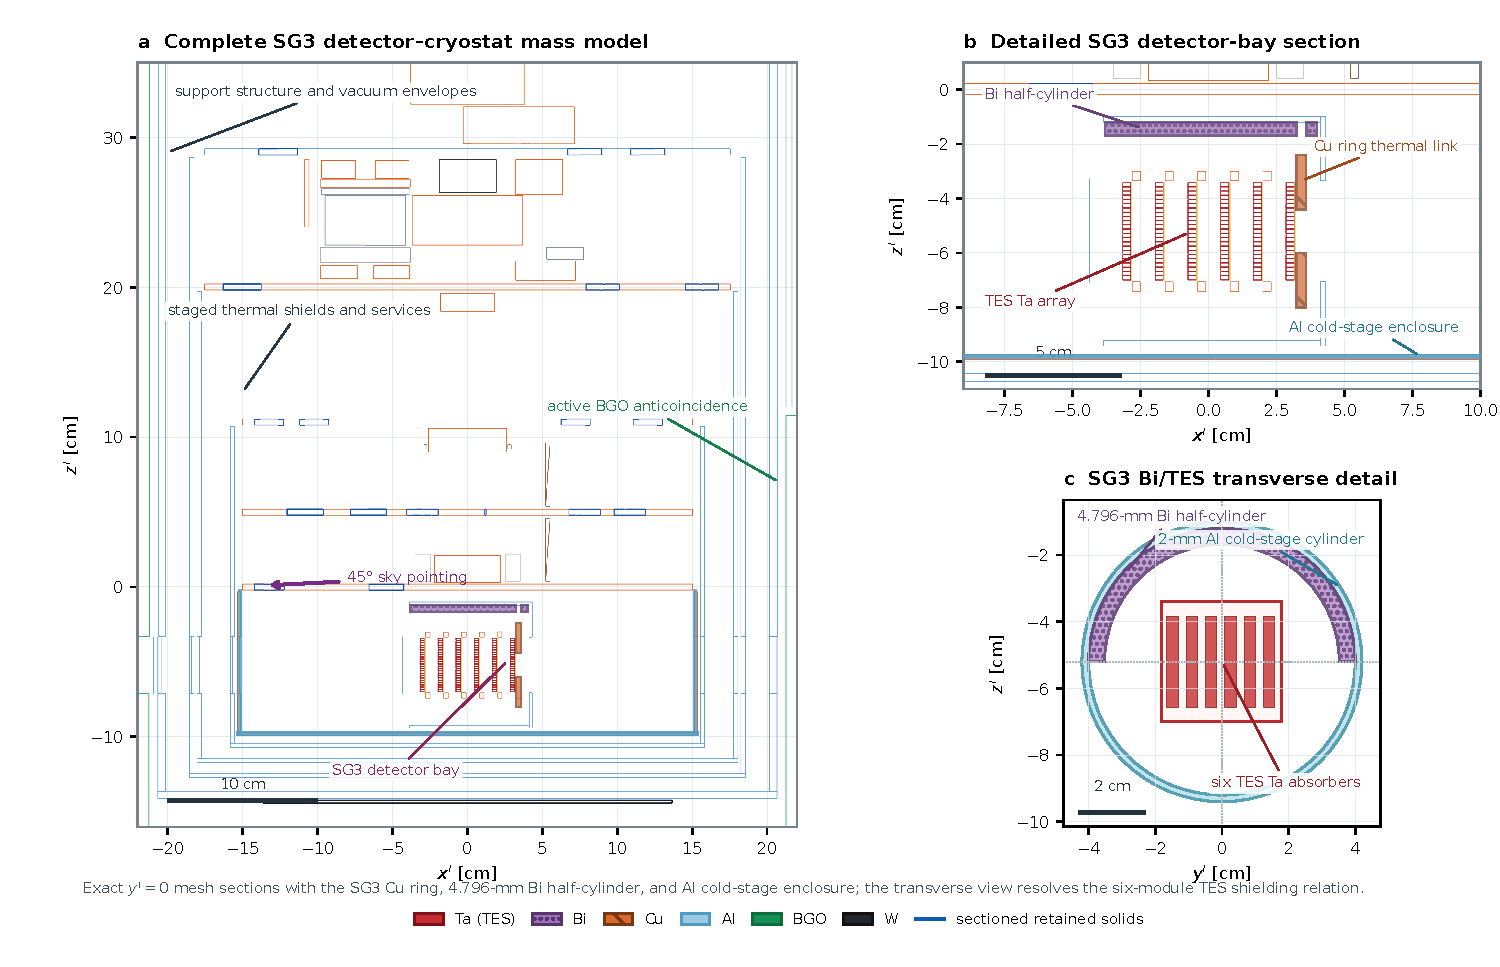
\includegraphics[width=0.98\linewidth]{figures/fig01_sg3_detailed_mass_model_en.pdf}
\caption{Current SG3 reference detector--cryostat mass model. (a) Exact global
$y'=0$ mesh section containing the support structure, vacuum envelopes, nested
thermal shields, active BGO, cold plates, and detector bay; the arrow marks the
fixed-$45^\circ$ sky-pointing direction. (b) Enlarged detector-bay section with
the six TES planes, Cu ring thermal link, Bi half-cylinder, and Al cold-stage
enclosure. (c) Section normal to the cylinder axis, resolving the 4.796-mm Bi
half-cylinder, 2-mm Al cylinder, and six TES Ta absorbers.}
\label{fig:mass_model}
\end{figure}

The mass-model section in Figure~\ref{fig:mass_model} is drawn from the retained
triangle mesh rather than from a reduced detector cartoon. The global panel
therefore keeps the vacuum enclosure, support shell, nested thermal shields,
service penetrations, active BGO, cold plates, and detector bay on one common
instrument coordinate system. The near-field panel resolves the components
that matter directly for the 511 keV background: the six Ta absorber planes,
their copper support and heat-sink connection, the aluminium cold enclosure,
and the bismuth member above the focal plane. In SG3 the latter is a
4.796-mm-thick upper half-cylinder nested immediately inside the retained
2-mm aluminium cylinder. This construction preserves a continuous optical
opening while avoiding the unphysical interpretation of a flat, infinite
absorber plate.

The three panels also separate two geometrical questions that enter the later
analysis. The global section establishes which massive payload structures can
produce or scatter particles into the cryostat, whereas the two near-field
sections establish which activated structures subtend the TES after production.
The selected-event provenance analysis uses the generated volume names and
coordinates associated with this same geometry, not hand-assigned radial
regions. Consequently, a delayed event attributed to a mixing-chamber plate,
a copper ring, or a TES-near member can be placed back into the geometry without
changing coordinate systems. This source--geometry correspondence is the
basis for distinguishing activity that is merely present in the payload from
activity that is efficiently coupled to the science window.

SG3 and SH3 retain the same six sensitive planes, pixel dimensions, response
model, entrance aperture, and optical-axis convention. The controlled change
is the relationship between the focal plane and the cold structures. In SG3
the TES lies underneath their projected area. In SH3 it lies along the lateral
chimney axis, behind a compact local frame and within an active-BGO envelope.
Keeping the detector and optical definitions fixed is essential: otherwise a
reduction in background could not be separated from a simultaneous loss of
focused acceptance.

\FloatBarrier

\section{Simulation framework}
\label{sec:framework}

Detector-coupled Monte Carlo transport through detailed mass models is a
mature method for predicting the response and background of gamma-ray
spectrometers \cite{Sturner2003}. The optics branch transports an on-axis 511 keV
point source through the Laue lens and records the focal-plane phase space. The
detector branch then treats three physical chains independently: the resulting
focused EventList, the corrected broadband atmospheric field, and radioactive
decays sampled from their recorded production positions. Activation production
is the source-building stage of the delayed chain rather than a counted prompt
component. All three chains receive the same pixel response, science window,
active BGO anticoincidence, and topology/field-of-view selection. Their selected
rates are placed on a common time axis and folded through the same 81-node
trajectory.

Figure~\ref{fig:workflow} retains the mature source-to-response logic while making
the present source contract explicit. The corrected broadband gamma tables
include the atmospheric annihilation feature, so no independent monoenergetic
atmospheric line is added. The source decomposition and mission fold then connect
the SG3 reference diagnosis to the SH3 side-chimney comparison. Day-scale flights
sample a continuum of atmospheric and geomagnetic states, so the trajectory fold
and its five common-time anchor calculations are developed in
Section~\ref{sec:mission_time_fold}.

\begin{landscape}
\centering
\vspace*{\fill}
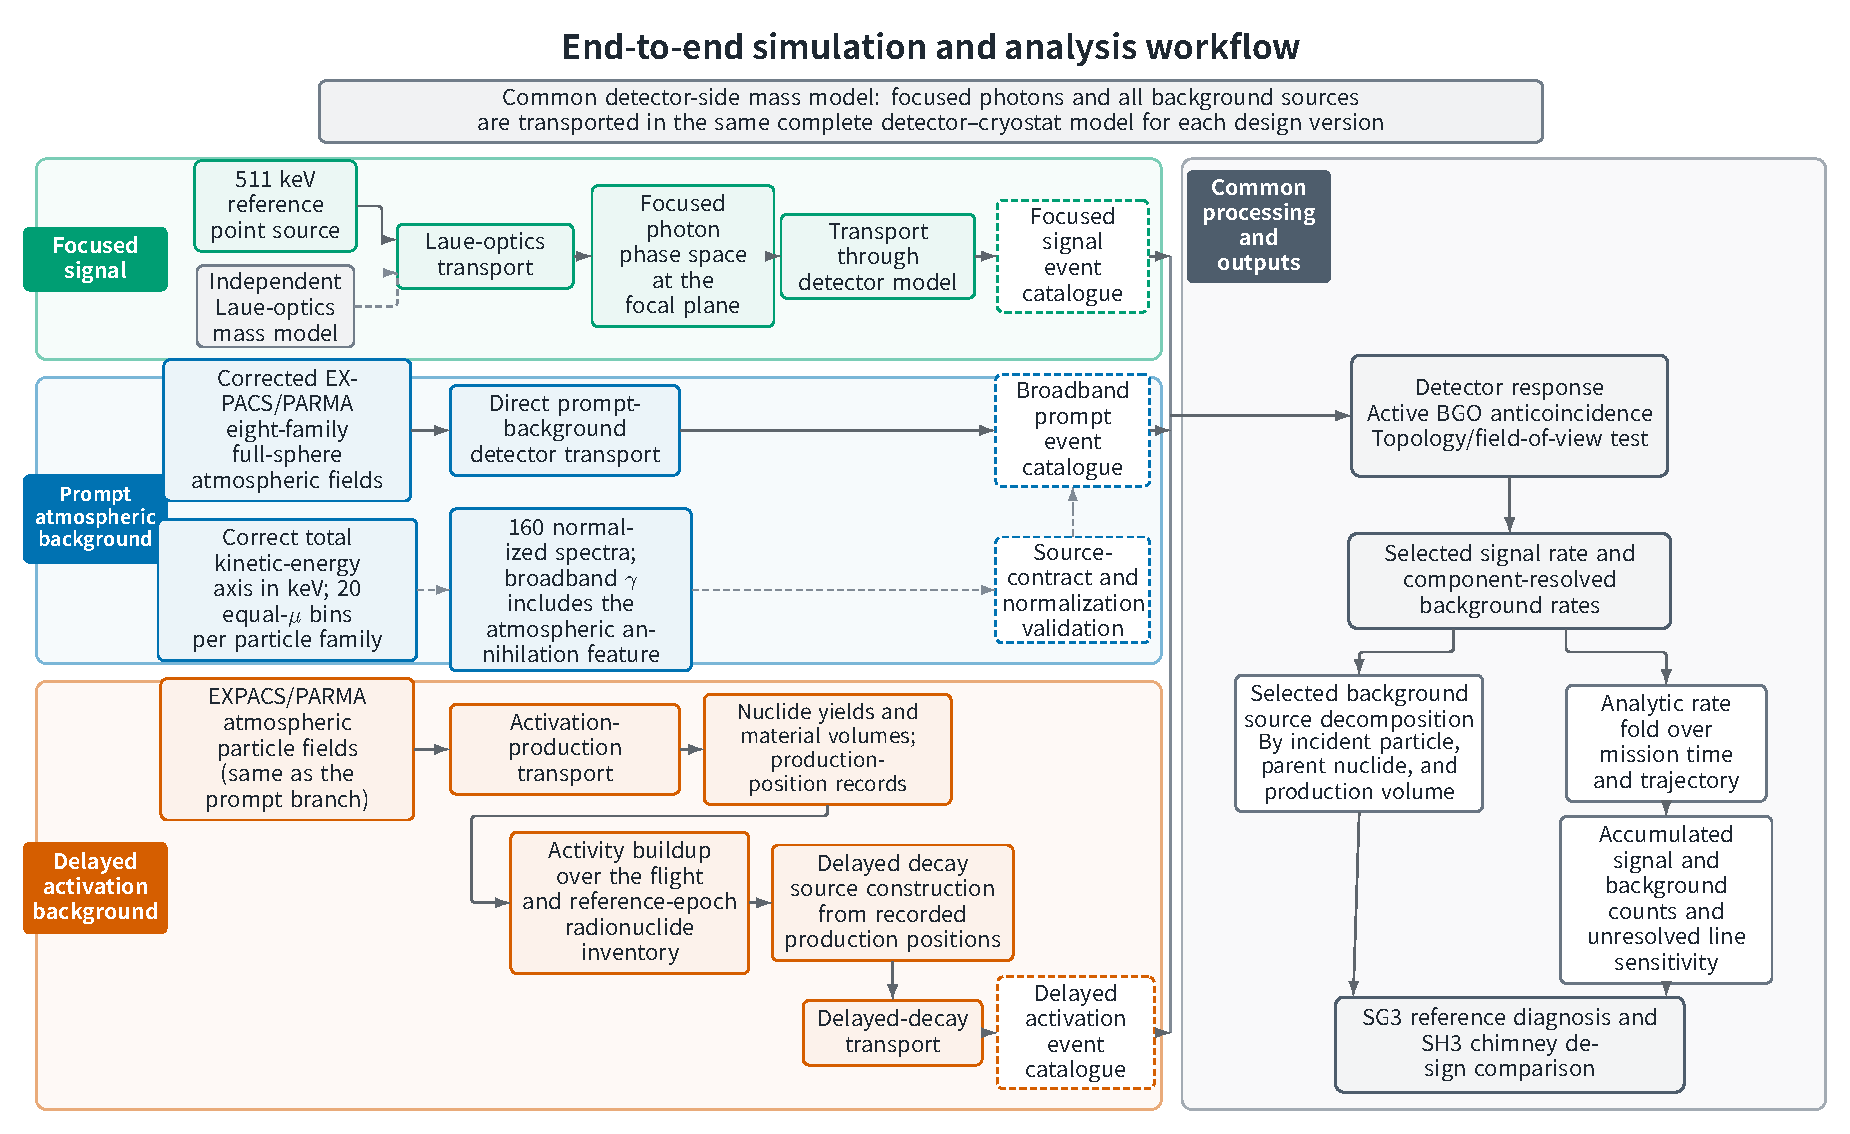
\includegraphics[width=0.94\linewidth]{figures/fig02_workflow_en.pdf}
\captionof{figure}{End-to-end simulation and analysis workflow. Focused signal,
the corrected eight-family atmospheric field, and production-position-sampled
activation decays are transported separately and then subjected to the common
detector response, science window, active BGO anticoincidence, and
topology/field-of-view selection. The selected rates enter source decomposition
and the 81-node mission fold used for the SG3--SH3 comparison.}
\label{fig:workflow}
\vspace*{\fill}
\end{landscape}

\FloatBarrier

\subsection{Laue optics and detector-coupled signal transport}
\label{sec:optics}

This simulation adopts a laue-lens system based on mosaic Ge(111) crystals \cite{Barriere2009Laue,Barriere2011LauePrototype}. Through optical design, it realizes a 10 m focal length, a 511\keV{} single-ring reference response, and an effective area of $20.1\,\mathrm{cm^2}$ at 511\keV; the effective area is calculated as
\begin{equation}
  A_{\mathrm{eff}}(E)=A_{\mathrm{inc}}\frac{N_{\mathrm{fp}}(E)}{N_{\mathrm{inc}}(E)}
  \label{eq:laue_aeff}
\end{equation}
where $A_{\mathrm{inc}}$ is the Monte Carlo incident sampling area, $N_{\mathrm{inc}}(E)$ is the number of incident photons, and $N_{\mathrm{fp}}(E)$ is the number of photons satisfying the focusing/focal-plane interception condition.
The mosaic system is adopted to make the Monte Carlo calculation convenient while satisfying the expected focusing performance; other candidate schemes are also possible for actual engineering adaptation.

In this simulation, the laue optical branch gives the focusing-performance simulation and transports the focused signal through the Ge crystal mass.

For this purpose, the diffraction probability of photons by the crystal is no longer superposed onto photons as an efficiency parameter, but is defined as a discrete process at the Geant4 application layer \cite{Agostinelli2003,Allison2016}. The process takes the diffraction probability $R(|\Delta\theta|)$ according to the angular deviation of the current photon relative to the crystal plane, and converts it into a finite equivalent diffraction mean free path $\lambda_{\mathrm{diff}}$, so that the accumulated diffraction probability when the photon crosses a crystal path $\ell$ reproduces this value: $1-\exp(-\ell/\lambda_{\mathrm{diff}})=R(|\Delta\theta|)$, namely $\lambda_{\mathrm{diff}}=-\,\ell/\ln[1-R(|\Delta\theta|)]$; to avoid double counting with standard photoelectric absorption, $R$ is first normalized by the unabsorbed fraction ($R/(1-A)$) and then converted into a mean free path. After this mean free path is returned to Geant4, the diffraction process and the standard electromagnetic processes (photoelectric absorption and Compton scattering) each sample interaction lengths in the same competition framework, and the shortest one decides which process occurs first, rather than forcibly intercepting photons at the crystal boundary. Photons not selected to undergo diffraction still continue transport according to the standard electromagnetic physics, and may be absorbed, scattered, or directly transmitted.

The diffraction probability is preferentially given by interpolation in an external XOP/CRYSTAL rocking-curve map as a function of angular deviation: this curve is calculated offline once in the preprocessing stage by the CRYSTAL/diff\_pat module of the XOP toolkit (called through xoppylib, with DABAX crystallographic data as input) \cite{SanchezDelRio2011XOP}, and gives the Ge(111) reflectivity/transmissivity/absorption curves as a function of angular deviation; during transport, the angular deviation is calculated in real time for every step inside the crystal, and the current diffraction probability is obtained by interpolation on that curve, namely ``offline library tabulation, probability used by angle during transport''. The mosaic orientation is implemented by applying a Gaussian angular perturbation to the ideal Bragg-plane normal, with the perturbation width given by the 30 arcsec mosaic FWHM; after diffraction occurs, the outgoing direction is mirror-reflected according to the perturbed plane normal, and the photon energy is unchanged. This split in which the ``process class only handles the transport interface, and the independent model class handles probability and direction decisions'' follows the idea of existing crystal Bragg-reflection extensions in Geant4 \cite{Guan2023BraggReflection,Reiazi2025G4BraggReflection}, and extends it to the energy band needed here.

Here the reference signal is a monochromatic 511\keV{} point source whose
rounded top-of-atmosphere flux scale
($\fzero=10^{-4}\phcms$, Section~\ref{sec:requirements}) is motivated by the
dedicated INTEGRAL/IBIS compact-source upper limit \cite{DeCesare2011}, rather
than by any single observed object. It is constructed as a MEGAlib far-field source
\cite{Zoglauer2006}, with the detailed construction given in
Section~\ref{subsec:pointsource}. The signal is transported through the optics
branch and injected into the detector mass model as a parallel-beam source;
prompt cosmic-ray background and activation decays are transported directly in
the detector/cryostat mass model. The primary background budget is therefore
defined for the detector/cryostat branch, while the optics branch supplies the
transported focal-plane signal phase space.

\subsection{Source construction}
\label{sec:background}

After the focusing optics have been defined in Section~\ref{sec:optics},
the calculation constructs the focused point source, the prompt atmospheric
field, and the delayed radioactive population independently. Activation
production and delayed-decay transport remain separate operations within the
delayed chain. This preserves the normalization and particle--nuclide--position
provenance of every component before the common detector response and event
selection are applied.

\subsubsection{Prompt atmospheric source}
\label{subsec:prompt_source}

The prompt atmospheric field is derived from EXPACS/PARMA. PARMA3.0 is an
analytical model parameterized from PHITS atmospheric-shower calculations and
benchmarked against terrestrial cosmic-ray measurements, and EXPACS is its
public tabulation and software interface
\cite{Sato2015EXPACS,Sato2016PARMA4}. PHITS supplies the underlying
particle-transport physics: primary cosmic rays interact with air nuclei, the
secondary hadrons, leptons, photons, and neutrons are transported through the
atmospheric column, and the resulting fluences are parameterized by altitude,
geomagnetic cutoff, solar modulation, energy, and direction. In this work
EXPACS/PARMA provides the differential incident flux as a function of particle
species, kinetic energy, zenith angle, geographic position, altitude, cutoff
rigidity, and solar activity, and is used only to construct the external
radiation fields; detector response, vetoing, topology selection, and
mission-time counting are applied downstream. The reference source definitions
use latitude $34^\circ$, longitude $100^\circ$, altitude $38\,\mathrm{km}$,
vertical cutoff rigidity $R_c=11.6\,\mathrm{GV}$, and the 2025-08-31 solar
condition corresponding to $W=118.3$.

The prompt source includes photons, neutrons, electrons, positrons, protons,
alpha particles, and negative and positive muons. For each particle family the
EXPACS/PARMA differential spectrum is converted into a MEGAlib far-field area
source covering the full zenith range $\theta=0^\circ$--$180^\circ$ and full
azimuth range $\phi=0^\circ$--$360^\circ$. The zenith dependence is represented
by 20 differential equal-$\mu$ angular bins, where $\mu=\cos\theta$ and each
bin subtends $\Delta\Omega=0.6283185307\,\mathrm{sr}$: the first ten bins cover
down-going particles, the last ten up-going or albedo-like particles. Both
hemispheres are retained in the prompt transport and in the
activation-production transport, so upward albedo particles are not discarded
at source construction. Figure~\ref{fig:expacs_fullsphere_flux} shows the
resulting full-sphere flux field.

\begin{figure}[t]
\centering
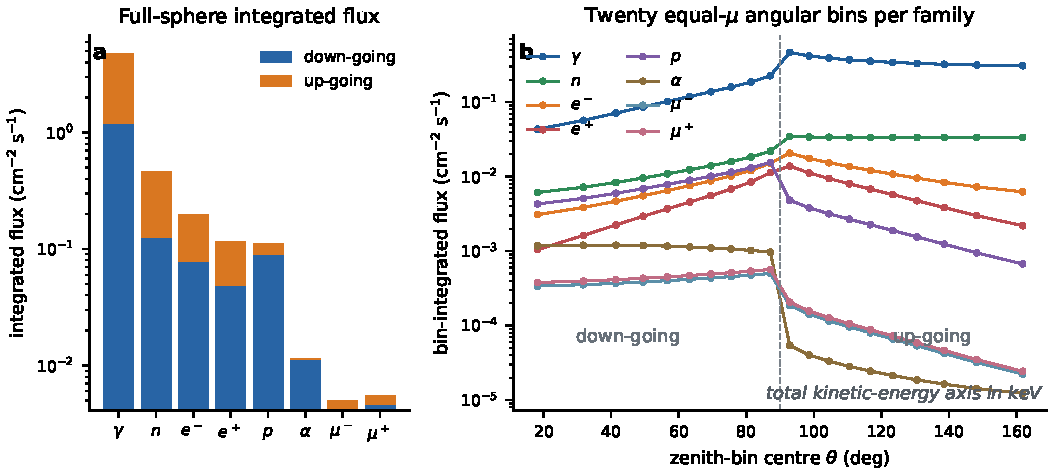
\includegraphics[width=\linewidth]{figures/fig03_corrected_kev_sources.pdf}
\caption{Corrected-total-kinetic-energy EXPACS/PARMA atmospheric field used for
prompt transport and activation production. (a) Energy- and solid-angle-integrated
fluxes of the eight particle families, separated into down-going and up-going
hemispheres. (b) Bin-integrated fluxes in the 20 equal-$\mu$ zenith bins used by
each far-field source. The environment is latitude $34^\circ$, longitude
$100^\circ$, altitude $38\,\mathrm{km}$, $R_c=11.6\,\mathrm{GV}$, and $W=118.3$.}
\label{fig:expacs_fullsphere_flux}
\end{figure}

The full-sphere integrated fluxes are 4.79966, 0.462239, 0.199002,
0.116981, 0.112301, 0.0114871, 0.00496893, and
$0.00557001\,\mathrm{cm^{-2}\,s^{-1}}$ for $\gamma$, $n$, $e^-$, $e^+$, $p$,
$\alpha$, $\mu^-$, and $\mu^+$, respectively. All families use 20 equal-$\mu$
angular bins and a 60 cm far-field start sphere. Minority families may be sampled
more heavily, but every family retains its own transported exposure,
\begin{equation}
  r_{\mathrm{event},j}=\left(\sum_i \mathcal{T}_{ij}\right)^{-1},
\end{equation}
where $\mathcal{T}_{ij}$ is the exposure of subsample $i$ for family $j$.
Consequently, over-sampling changes Monte Carlo variance but not the expected
physical rate.

The energy axis supplied to Cosima is total kinetic energy in keV: for non-alpha
families $E_{\mathrm{tot,keV}}=1000E_{\mathrm{MeV}}$, while for alpha particles
$E_{\mathrm{tot,keV}}=4\times1000E_{\mathrm{MeV/nucleon}}$. The retained source
package contains 160 normalized spectra (20 per family) and 24 geometry-specific
source cards. Their numerical integrals span
$0.999999999991$--$1.000000000006$, and all 480 spectrum references resolve to
the corrected energy contract.

The angular and energy normalizations are deliberately factored. If
$I_j(E,\mu)$ denotes the EXPACS/PARMA differential intensity for family $j$,
the flux carried by equal-$\mu$ bin $m$ is
\begin{equation}
 \Phi_{j,m}=2\pi\int_{\mu_m}^{\mu_{m+1}}\!\mathrm d\mu
             \int I_j(E,\mu)\,\mathrm dE,
 \qquad \Delta\mu=0.1,
 \label{eq:source_bin_flux}
\end{equation}
so every bin subtends $\Delta\Omega=2\pi\Delta\mu=0.62831853\,\mathrm{sr}$.
The first ten bins cover the down-going hemisphere and the second ten cover the
up-going or albedo hemisphere; azimuth is complete in both cases. The spectrum
within each bin is normalized to unit integral, while $\Phi_{j,m}$ carries the
physical amplitude. This separation prevents a spectral-table normalization
from being mistaken for a particle flux.

All eight families use the same 60 cm enclosing source sphere and the same
directional convention. For a sampled direction, the source implementation
draws the starting point on the corresponding projected disk and points the
momentum into the enclosed mass model. Thus the geometrical rate factor is the
projected area $\pi R^2$, not the surface area $4\pi R^2$. Full-sphere in this
context means complete incident solid angle; it does not mean uniform emission
from arbitrary points on a spherical shell. The distinction is important for
both prompt transport and activation production because an area error would
propagate linearly into every derived rate and activity.

The corrected energy convention is likewise applied before any transport
normalization. Electrons, positrons, photons, nucleons, and muons use the
tabulated kinetic energy multiplied by $10^3$ to convert MeV to keV. The alpha
tables are per nucleon and therefore require the additional mass-number factor
of four. Applying the same numerical conversion to alpha particles and the
other seven families would shift their kinetic-energy distribution by another
factor of four; treating the tabulated MeV values as keV would shift all
families by three decades. The source contract records these two cases
explicitly rather than relying on an implicit unit convention.

The retained package-level checks test the quantities that enter the physics
normalization. There are 20 spectra for each of eight families, every spectrum
is finite and non-negative, every numerical integral is unity to the precision
quoted above, and every source-card reference resolves to the corrected-keV
set. The geometry header of a source card must also agree with the mass model
used by its transport. Prompt and activation-production inputs share the same
field definition but remain separate calculations, so an activation product is
never counted once as an immediate detector event and again as a later decay.

This construction also defines what can and cannot be inferred from the photon
component. Its $4.79966\,\mathrm{cm^{-2}\,s^{-1}}$ integral is the broadband
full-sphere photon flux across the retained energy domain. The table contains
the annihilation enhancement and its adjacent continuum with their original
energy dependence. The detector science-window rate is therefore obtained by
transporting and response-convolving that broadband component; it is not the
product of an independently fitted line flux and a detector efficiency. This
avoids both double counting and an artificial separation of photons that are
indistinguishable at the source-contract level.

\subsubsection{Broadband atmospheric gamma component}
\label{subsec:atm511_source}

The corrected atmospheric photon tables are treated as a single broadband gamma
component. Their retained spectrum contains the annihilation feature around
511 keV together with the surrounding continuum. Adding a separate monoenergetic
atmospheric source would therefore count the same physical feature twice. The
gamma component instead follows the same 20-bin full-sphere geometry, exposure
normalization, detector response, and trajectory-dependent family scaling as the
other seven atmospheric families.

This contract preserves the distinction between the celestial signal and local
atmospheric photons without introducing a second atmospheric-line normalization.
The science signal remains the focused, on-axis EventList; atmospheric gamma
events enter only through the broadband prompt catalogue and are decomposed by
their incident-family tag after selection.

\subsubsection{Delayed activation source}
\label{subsec:delayed_source}

The delayed source is built from a separate activation-production transport. It
is not counted as immediate detector background; instead, it records the isotope,
material volume, incident family, and production position of each radioactive
product. Ground-state half-lives are checked against NUBASE2020
\cite{Kondev2021NUBASE}. For isotope $k$,
\begin{equation}
  A_k(t_{\mathrm{flight}})=P_k\left[1-\exp(-\lambda_k t_{\mathrm{flight}})\right],
  \qquad \lambda_k=\frac{\ln2}{t_{1/2,k}},
\end{equation}
where $P_k$ is the production rate and the reference state is
$t_{\mathrm{flight}}=15\,\mathrm{d}$. The resulting all-family day-15 activities
are $1352.29749\,\mathrm{Bq}$ for SG3 and $211.387433\,\mathrm{Bq}$ for SH3.

An aggregate inventory alone is insufficient for this construction. The
production calculation therefore retains a coordinate record at the moment a
radioactive product is created, and the day-15 population is matched to those
records by material volume, nuclide, and excitation state. The resulting source
description is indexed by incident family, material category, production volume,
and coordinate. These are source-construction quantities rather than detector
counts: attenuation, decay transport, detector response, and event selection are
applied only after the delayed particles are emitted from their recorded
locations in the common geometry.

Position information is retained because downstream attenuation, active-shield
probability, and topology depend on where a radionuclide was created. Production
records are matched by volume, nuclide, excitation state, and coordinate before
decay transport. The activity-normalized material distributions of incident
families $a$ and $b$ may be compared through
\begin{equation}
  D_{\mathrm{TV}}(a,b)=\frac12\sum_c|f_{a,c}-f_{b,c}|,
\end{equation}
where $f_{a,c}$ is the fraction of family-$a$ activity in material category $c$.
This provenance is essential: a volume-integrated source could preserve total
activity while erasing the family--material--nuclide correlations that determine
the selected science-window background.

Let production row $j$ carry activity weight $w_j$, with
$A=\sum_jw_j$. Drawing $M$ production positions with replacement using
$p_j=w_j/A$ and assigning each point source flux $A/M$ gives
\begin{equation}
  \mathbb{E}\!\left[N_j\frac{A}{M}\right]=Mp_j\frac{A}{M}=w_j,
\end{equation}
so the sampled source is unbiased and conserves total activity. Each current
family catalogue transports $10^6$ delayed decays. The SH3 realization therefore
contains $8\times10^6$ delayed triggers and retains 111 delayed records after the
complete science-window, BGO, and topology selection. Its day-15 activities by
incident family are 34.2836, 0.2663, 0.6754, 2.0320, 0.0684, 0.0040, 68.5316,
and 105.5262 Bq for $\alpha$, $e^-$, $e^+$, $\gamma$, $\mu^-$, $\mu^+$, $n$,
and $p$.

Table~\ref{tab:background_source_model} summarizes the source layers. Source
construction ends before detector response, anticoincidence, and topology
selection; the latter operations are defined in Section~\ref{sec:selection}.

\begin{table}[t]
\centering
\caption{Source layers used by both geometries. The table defines source
construction; detector response and selection are applied downstream.}
\label{tab:background_source_model}
\footnotesize
\begin{tabular}{p{0.21\linewidth}p{0.34\linewidth}p{0.37\linewidth}}
\toprule
Layer & Physical role & Current implementation \\
\midrule
Corrected atmospheric field & Prompt detector hits and activation production &
Eight families, 20 equal-$\mu$ bins per family, full sphere, 60 cm start radius;
correct total kinetic energy in keV. \\
Broadband gamma & Atmospheric photons including the annihilation feature &
One retained broadband component; no additive monoenergetic normalization. \\
Activation production & Family--nuclide--volume--position history &
The same corrected atmospheric field, with NUBASE-checked ground-state decay data. \\
Day-15 radioactive population & Flight-time activity used for delayed transport &
SG3: $1352.29749\,\mathrm{Bq}$; SH3: $211.387433\,\mathrm{Bq}$. \\
Production-position decay & Delayed particles emitted from recorded material coordinates &
$10^6$ decays per family; eight independently normalized family catalogues per geometry. \\
\bottomrule
\end{tabular}
\end{table}

The selected delayed events retain their source-parent identity and exact
production volume. In SG3, the leading groups include $^{62}$Cu in an L2 copper
support ring and in the 50 mK mixing-chamber plate. In SH3, the largest group is
$^{62}$Cu in an L5 copper ring, followed by $^{62}$Cu in the TES heat-sink ring;
tungsten-frame and aluminium-shell groups are smaller. These selected-event
origins, rather than the unfiltered total inventory alone, drive the geometry
interpretation in Section~\ref{subsec:reference_background_results}.

\subsubsection{Reference point-source construction}
\label{subsec:pointsource}

The focused signal stream is defined by a monochromatic 511\keV{} reference
point source. Its flux scale is set not by any single observed object but by a
rounded comparison to the dedicated INTEGRAL/IBIS compact-source limit:
$\fzero=10^{-4}\phcms$ at the top of the atmosphere
(Section~\ref{sec:requirements}) \cite{DeCesare2011}.

Because such a source lies at astronomical distance, it is modelled as an ideal
on-axis point: in the optics calculation it is a monochromatic 511\keV{}
far-field beam whose photons arrive parallel to the optical axis and are sampled
uniformly over the incident aperture $A_{\mathrm{inc}}$ of
Equation~(\ref{eq:laue_aeff}). No finite angular size is assigned to the source
itself. The angular structure at the focal plane is produced by the 30 arcsec
mosaic spread, the XOP/CRYSTAL rocking curve, and the 10 m focusing geometry, so
the accepted photons form a finite spot rather than a single ray. Three
independent optics samples totalling $1.5\times10^5$ incident photons yield 37,256
diffracted focal-plane crossings; 37,194 of them fall inside the
$r=1.898\,\mathrm{cm}$ beryllium entrance window. Their spot radii are
$r_{90}=1.03\,\mathrm{cm}$ and $r_{99}=1.25\,\mathrm{cm}$. The recorded position
and direction of each accepted crossing form the common detector-side EventList
used for both geometries.

The focused rate at the detector entrance is
\begin{equation}
  R_{\mathrm{fp}}=F_{\mathrm{TOA}}\,\aeff(511\keV)\,T_{\mathrm{atm},45}.
\end{equation}
Equivalently, the generating optics sample represents an exposure
$N_{\mathrm{fp}}/[F_{\mathrm{TOA}}\aeff T_{\mathrm{atm},45}]$, and every
EventList entry carries the inverse of that exposure as its physical rate
weight. This separates detector-side acceptance from the top-of-atmosphere flux
normalization and applies the latter only once. Because the optics calculation
contains source photons only, all backgrounds still enter exclusively through
the atmospheric and delayed-activation streams defined above.
Here $T_{\mathrm{atm},45}=0.652034$ at day 15. In SG3, 28,612 entries lie in the
measured science window and 28,006 pass the final topology selection, giving
$A_{\mathrm{eff}}=15.12324\pm0.04492\,\mathrm{cm^2}$. In SH3 the corresponding
counts are 28,434 and 27,936, giving
$15.08544\pm0.04503\,\mathrm{cm^2}$. After atmospheric transmission and the
day-15 accidental-coincidence survival are applied, the rates at
$F_{\mathrm{TOA}}=10^{-4}\phcms$ are $9.5362\times10^{-4}\cps$ for SG3 and
$9.7904\times10^{-4}\cps$ for SH3. Thus the chimney changes the selected area by
only $0.25\%$ while substantially changing the background environment.

The effective area quoted above is the on-axis value, representing best-case
pointing. A point source offset from the optical axis, or residual attitude
jitter during flight, reduces and shifts the focused response through the finite
angular acceptance (field of view) of the Laue lens
\cite{Barriere2009Laue,Weidenspointner2006MAX}; this off-axis dependence is
treated as a pointing systematic on the signal effective area rather than as a
change to the on-axis reference construction. The current side-entry response
is a fixed $45^\circ$-elevation reference, not a simulated
low-elevation Galactic-centre observation.

\subsection{Background-led geometry design and statistical treatment}
\label{subsec:comparison_hierarchy}

The design starts from events that reach the science window. For SG3, final
prompt events are grouped by incident family and delayed events by incident
family, source-parent nuclide, production material, volume, and coordinate. This
component-first logic follows detailed COSI and DIXE background studies
\cite{Gallego2025Balloon,Tian2026DIXE}. It shows that the staged cold region lies
directly over the SG3 focal plane. SH3 therefore translates the TES laterally
into the side chimney while retaining the optical acceptance and surrounding the
new focal region with active BGO.

Cosima deposits are aggregated by TES pixel before an independent Gaussian
response with $\Delta E_{\mathrm{FWHM}}=0.420\keV$
($\sigma=0.17836\keV$) is applied. Measured hits below 0.300\keV{} are removed,
and the remaining hits are summed before the science-window, BGO, and topology
tests. All geometry comparisons use this identical response contract.

For stream $k$ and stage $j$, the physical rate, Monte Carlo standard error, and
effective support are
\begin{equation}
  \widehat R_{k,j}=\sum_{i\in(k,j)}w_i,\qquad
  \sigma_{k,j}=\left(\sum_{i\in(k,j)}w_i^2\right)^{1/2},\qquad
  N_{\mathrm{eff},k,j}=\frac{\widehat R_{k,j}^2}{\sigma_{k,j}^2}.
  \label{eq:weighted_rate_stats}
\end{equation}
Counts report transported support, whereas weighted rates report the physical
background. We also retain the stage survival
$q_{k,j}=\widehat R_{k,j}/\widehat R_{k,\mathrm{window}}$ and the final component
share $f_k=\widehat R_{k,\mathrm{final}}/\sum_b\widehat
R_{b,\mathrm{final}}$, because a small transported count can still carry an
important physical rate when component exposures differ.

Within an independently normalized transported component the event weights are
constant, so a two-sided 95\% Garwood interval for the Poisson count can be
multiplied by the component weight to give an exact rate interval. A zero selected
count with defined exposure therefore gives an upper limit rather than a claim of
zero physical background. Focused-signal acceptance is binomial and is checked
with the corresponding exact interval. These componentwise bounds diagnose finite
transport support; they are not a joint-coverage band and do not include radiation
field, cross-section, calibration, or pointing systematics. The primary mission
uncertainty instead propagates the background-transport, common-time replay,
selected-area, and accidental-probe terms by the delta method.

For trajectory bin $\ell$, live fraction $L_\ell$, and duration $\Delta t_\ell$,
\begin{equation}
 N_s(T)=\sum_{\ell\le T}S_\ell L_\ell\Delta t_\ell,\qquad
 N_b(T)=\sum_{\ell\le T}B_\ell L_\ell\Delta t_\ell.
 \label{eq:cumulative_counts}
\end{equation}
We report both the Gaussian counting measure
$Z_G=N_s/\sqrt{N_b}$ and the Asimov form
\begin{equation}
 Z_A=\sqrt{2\left[(N_s+N_b)\ln\left(1+\frac{N_s}{N_b}\right)-N_s\right]}.
\end{equation}
The minimum flux is obtained from the same signal kernel by solving for
$Z=3$ or 5. This keeps the mission comparison on one statistical and physical
normalization.

\subsection{Detector event selection and veto definitions}
\label{sec:selection}

The focused-signal, prompt-atmospheric, and delayed-activation catalogues
are placed on one explicit time axis. The same measured science window, active
BGO anticoincidence, and topology/field-of-view definition is then applied to
both geometries. Prompt gamma already carries the retained atmospheric
annihilation feature, so the rate budget contains no additional atmospheric
catalogue.

\subsubsection{Time axis and rate normalization}

Each stream enters with a per-record rate weight $r_{km}$, with total
$R_k=\sum_mr_{km}$. For a reference interval $T$, independent Poisson draws
\begin{equation}
 N_k\sim\mathrm{Pois}(R_kT)
\end{equation}
are sampled with probabilities $r_{km}/R_k$, assigned uniform times in $[0,T]$,
merged, and ordered. Records separated by at most $\tau=1\,\mu\mathrm{s}$ form
one coincidence group. Five $2\times10^5$ s anchor realizations at days 0, 5,
10, 15, and 20 test this construction. Figure~\ref{fig:s33_poisson} compares the
common-time rate with the independently normalized direct rate, while
Figure~\ref{fig:s33_spec_norm} shows the weighted pre-veto spectra of the two
geometries. At day 15 the common-time/direct ratios are 0.9665 for SG3 and
1.0172 for SH3, consistent with the finite anchor counts; the corresponding
signal accidental-survival factors are 0.967071 and 0.995341.

\begin{figure}[t]
\centering
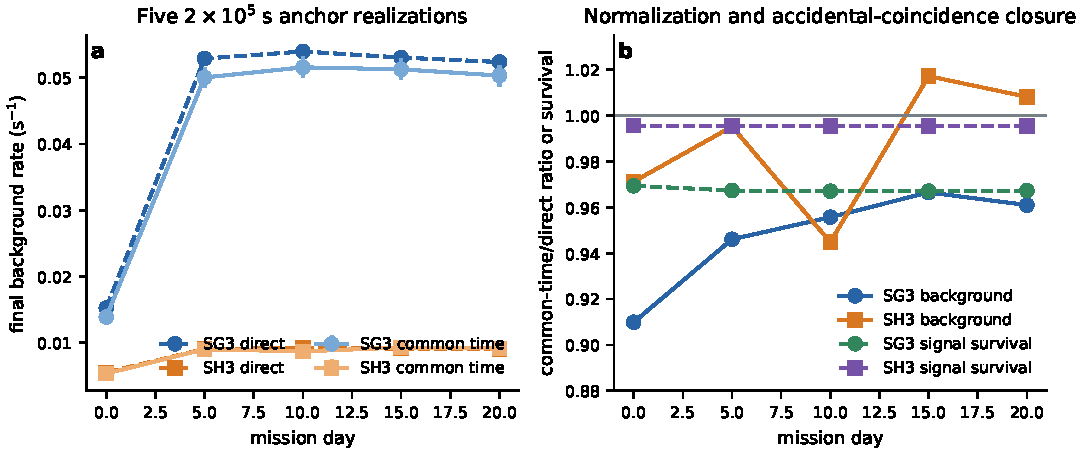
\includegraphics[width=\linewidth]{figures/fig04_common_time_normalization.pdf}
\caption{Common-time normalization at five mission anchors. (a) Direct
no-coincidence and $2\times10^5$ s common-time final background rates for SG3 and
SH3; error bars are Poisson standard errors of the anchor realization. (b)
Common-time/direct background ratios and focused-signal accidental-survival
factors. The same $1\,\mu\mathrm{s}$ grouping contract is used at all anchors.}
\label{fig:s33_poisson}
\end{figure}

\begin{figure}[t]
\centering
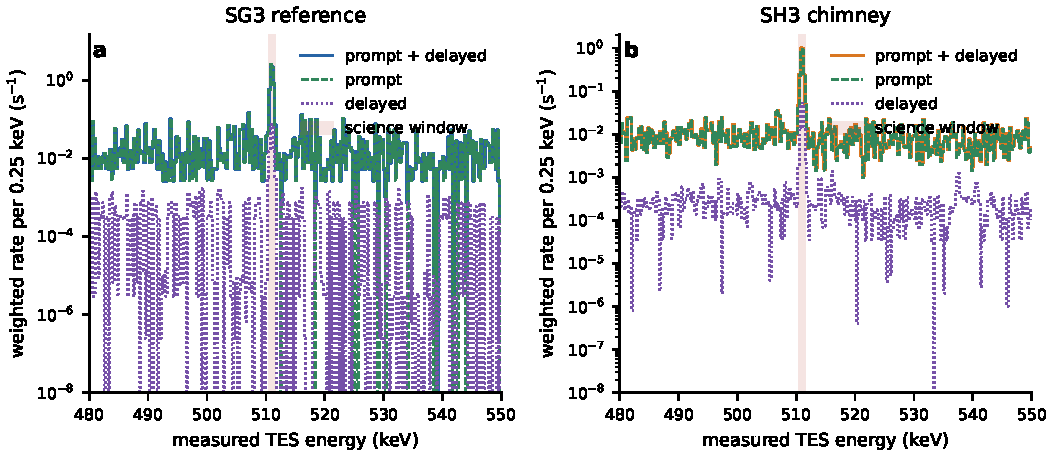
\includegraphics[width=0.82\linewidth]{figures/fig05_pre_veto_spectra.pdf}
\caption{Response-convolved, weighted prompt-plus-delayed spectra before active
vetoes for (a) the SG3 reference geometry and (b) the SH3 chimney geometry. The
shaded band marks the $510.58$--$511.42\keV$ science window; absolute cut-flow
rates are reported in Tables~\ref{tab:phase2_cutflow} and
\ref{tab:optimized_cutflow}.}
\label{fig:s33_spec_norm}
\end{figure}

The mission fold uses the common-time expectation in each trajectory bin,
\begin{equation}
 L_\ell=\exp\!\left\{-\tau\left[R^{\mathrm{occ}}_{\mathrm{prompt},\ell}+
 R^{\mathrm{occ}}_{\mathrm{delayed},\ell}\right]\right\}.
 \label{eq:common_live_factor}
\end{equation}
The weak focused source is excluded from the exponent; a brighter-source
application would add its occupancy explicitly. Atmospheric and activation rates
vary on mission-day scales, whereas grouping acts on microseconds, so each time
bin is treated as a stationary superposition. The five explicit anchors validate
the coincidence construction; the 81-node fold uses its expectation rather than
drawing a new stochastic realization in every bin.

\subsubsection{Active anticoincidence gate}

The first layer is active BGO anticoincidence. For coincidence group $c$,
\begin{equation}
 E_{\mathrm{TES}}^{(c)}=\sum_{j\in c}E_{\mathrm{TES},j},\qquad
 E_{\mathrm{sh}}^{(c)}=\sum_{j\in c}E_{\mathrm{sh},j}.
\end{equation}
The group enters the science window when
\begin{equation}
 \wii=[510.58,511.42]\keV
\end{equation}
and passes the active shield when
\begin{equation}
 E_{\mathrm{sh}}^{(c)}<E_{\mathrm{veto}},\qquad E_{\mathrm{veto}}=50\keV.
\end{equation}
In the SG3 direct catalogue, the gate changes the prompt sample from 1083 records
and $5.79018\cps$ to seven records and $1.87041\times10^{-2}\cps$, and the
delayed sample from 1295 records and $0.169494\cps$ to 436 records and
$4.34116\times10^{-2}\cps$. All 28,612 signal records in the measured window
pass active anticoincidence. Figure~\ref{fig:s33_spec_anti} shows the still
stronger SH3 BGO suppression.

\begin{figure}[t]
\centering
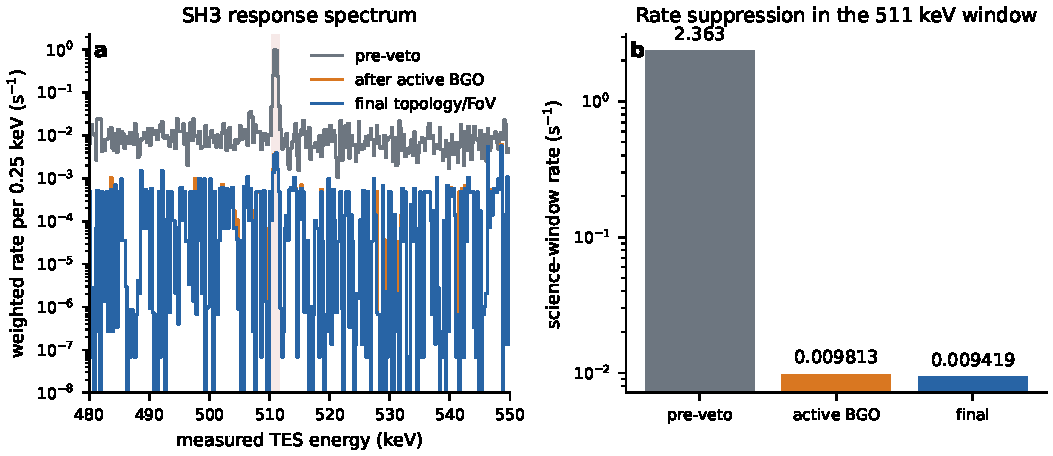
\includegraphics[width=0.82\linewidth]{figures/fig06_bgo_veto_spectrum.pdf}
\caption{Active-BGO suppression in the SH3 chimney geometry. (a) Weighted
480--550 keV spectra before anticoincidence, after active BGO, and after the final
topology/field-of-view selection. (b) Corresponding rates in the science window;
active BGO reduces the direct background from $2.36263$ to
$9.8133\times10^{-3}\cps$.}
\label{fig:s33_spec_anti}
\end{figure} The quoted flux thresholds apply to a line
whose intrinsic width, after detector response, remains small compared with this
window; a substantially broadened source line would require convolving the
source line profile with the response and re-optimizing the window.

\subsubsection{Compton topology and field-of-view consistency}

The second layer applies a Compton-kinematic topology and field-of-view
consistency test to the TES hits that survive the active-shield gate; its
physical basis is Compton-camera cone reconstruction \cite{Zoglauer2006}. An
incident photon of energy $E_0$ Compton-scatters at a first interaction point
$\mathbf r_1$, depositing $E_1$, and the scattered photon of energy
$E_{\mathrm{sc}}=E_0-E_1$ propagates to a second interaction point $\mathbf r_2$;
the scattering angle follows from
\begin{equation}
  \cos\theta_C =
  1 - m_ec^2\left(\frac{1}{E_{\mathrm{sc}}}
  - \frac{1}{E_1+E_{\mathrm{sc}}}\right).
\end{equation}
Given the scattered-photon direction
$\hat{\mathbf u}_{12}=(\mathbf r_2-\mathbf r_1)/|\mathbf r_2-\mathbf r_1|$, the
source direction is constrained to a reconstruction cone with apex $\mathbf r_1$,
axis $-\hat{\mathbf u}_{12}$, and half-angle $\theta_C$, whose projection on the
sky is the event circle. We use this first-scatter cone as an aperture-consistency
test: the event is retained when the cone intersects the side Be-window disk (radius
$1.898\,\mathrm{cm}$), i.e.\ whether the reconstructed arrival direction is
consistent with entry through the aperture.

Because the interaction position within a single TES pixel
($1.5\times1.5\times3.0\,\mathrm{mm}$) is unresolved, each hit is represented not
by its centroid alone but by $8+1=9$ representative points---the eight pixel
corners and the centroid---carrying the sub-pixel position uncertainty
explicitly into the geometric reconstruction. A two-hit event in a given scatter
order therefore enumerates $9\times9=81$ first/second position combinations and
constructs one reconstruction cone per combination (each cone sampled at 24
azimuths, propagated to the Be-window plane, and tested against the disk by both
its sampled points and the connecting segments); the order is deemed
field-of-view consistent if any of these 81 trajectories yields a cone that
intersects the disk. This is a deliberately permissive consistency test: an
event is retained if any sub-pixel interaction position is consistent with entry
through the aperture. The layer consequently retains about $95\%$ of the
in-window multi-hit events and removes only about $10$--$14\%$ of the background,
consistent with its role as a loose consistency veto rather than an imaging
reconstruction.

The three event classes are handled accordingly. Single-pixel events are
retained as calorimetric candidates. For two hits, both interaction orders and
the representative sub-pixel positions are tested, and either consistent order
is sufficient. For three to six hits, all orders are ranked by the Compton
sequence residual
\begin{equation}
 Q=\sum_{i=1}^{n-2}\left(\cos\theta_{C,i}-
 \hat{\mathbf u}_{i-1,i}\!\cdot\!\hat{\mathbf u}_{i,i+1}\right)^2,
\end{equation}
and the best order is subjected to the same cone--aperture test. The SG3 topology
layer retains 400 of 443 active-veto background records, with a weighted-rate
survival of $87.41\%$, and 28,006 of 28,612 signal records. In SH3 it retains
123 of 134 background records, with $95.98\%$ weighted-rate survival, and 27,936
of 28,434 signal records. Figure~\ref{fig:s33_compton_mult} resolves these samples
by TES hit multiplicity.

\begin{figure}[t]
\centering
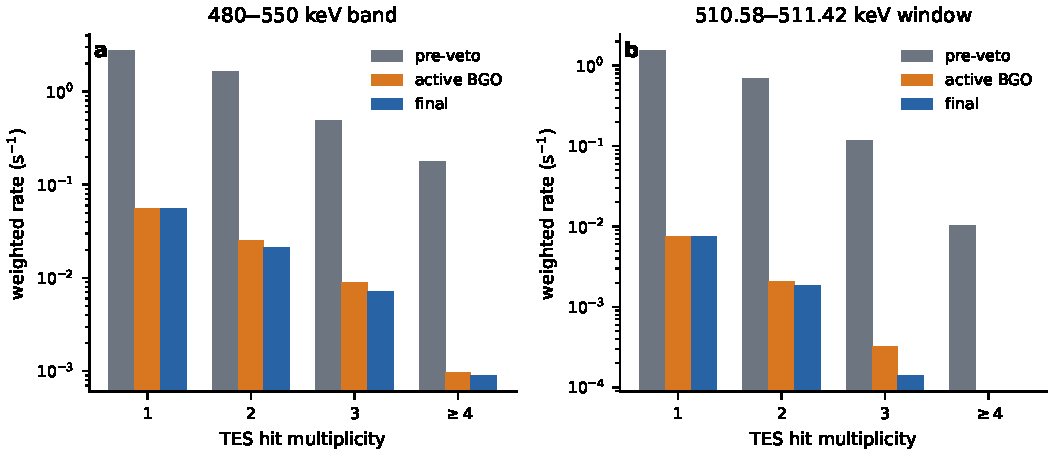
\includegraphics[width=\linewidth]{figures/fig07_hit_multiplicity.pdf}
\caption{SH3 weighted background rate by TES hit multiplicity before active
veto, after active BGO, and after topology/field-of-view selection in (a) the
480--550 keV band and (b) the $510.58$--$511.42\keV$ science window. Multi-hit
events are retained when their Compton cone is consistent with the entrance
aperture.}
\label{fig:s33_compton_mult}
\end{figure}

Unreconstructed events remain in the rate accounting but are not labelled
as field-of-view-consistent candidates. The measured multiplicity distributions
show why a permissive policy is appropriate: active BGO supplies the large rate
reduction, whereas topology removes a smaller residual population while
preserving the focused multi-hit signal. Table~\ref{tab:phase2_cutflow} gives the
SG3 reference cut-flow on the direct, no-coincidence normalization; its mission
rate is obtained from the common-time fold.

\begin{table}[t]
\centering
\caption{SG3 reference-geometry science-window cut-flow. Background entries are
direct no-coincidence counts/rates; signal entries give counts/effective area for
the common 37,194-ray focal sample.}
\label{tab:phase2_cutflow}
\footnotesize
\begin{tabular}{lccc}
\toprule
Stream & Pre-veto & After active veto & Final topology/FoV \\
\midrule
Prompt background & 1083 / $5.79018\cps$ & 7 / $1.87041\times10^{-2}\cps$ & 6 / $1.60321\times10^{-2}\cps$ \\
Delayed activation & 1295 / $0.169494\cps$ & 436 / $4.34116\times10^{-2}\cps$ & 394 / $3.82661\times10^{-2}\cps$ \\
Total background & 2378 / $5.95968\cps$ & 443 / $6.21157\times10^{-2}\cps$ & 400 / $5.42982\times10^{-2}\cps$ \\
Focused signal & 28612 / $15.45048\,\mathrm{cm^2}$ & 28612 / $15.45048\,\mathrm{cm^2}$ & 28006 / $15.12324\,\mathrm{cm^2}$ \\
\bottomrule
\end{tabular}
\end{table}

The retained hit-level catalogues provide an internal check of this
classification without another transport. For each selected event they preserve
measured hit energy, TES layer, pixel position, and multiplicity. Re-evaluating
the broad and science windows from these fields reproduces the tabulated stage
counts and confirms that the topology layer is applied after, rather than folded
into, the active-BGO decision.

\subsection{Mission-time trajectory and analytic rate folding}
\label{sec:mission_time_fold}

MeV balloon observations are background dominated: atmospheric secondaries and
cosmic-ray-induced activation set the rate floor, and both respond to the flight
environment \cite{Gallego2025Balloon,Kierans2017}. Detector-coupled Monte Carlo
through a fixed geometry provides the selected day-15 signal and background
rates under a common response, veto, and energy window, but those rates describe
only one longitude, latitude, and altitude. During a multi-day float the residual
atmospheric depth, geomagnetic cutoff, and activation inventory evolve, so a
constant-rate extrapolation of the day-15 snapshot is not a substitute for a
trajectory fold. We therefore map the reference rates onto a continuous 20 d
performance estimate and retain explicit common-time anchors as an independent
check of the time-axis construction.

The adopted trajectory is a \emph{synthetic reference profile}, not balloon
telemetry and not a source-visibility schedule. It contains 81 nodes from day 0
to day 20 at 0.25 d spacing, with a mild mid-latitude float envelope around
38.75 km altitude, $34^\circ$ latitude, and $100^\circ$ longitude. Altitude is
retained because changes in residual atmospheric depth affect both the particle
spectra that drive prompt background and activation and the 511\,keV atmospheric
transmission multiplying the focused signal. Latitude and longitude supply a
controlled reference modulation of the geomagnetic environment; they do not
encode Earth occultation, repointing losses, or the visibility of a named source.
The fold is therefore a reference-exposure sensitivity calculation rather than a
forecast for a particular launch campaign.

The fold contains five physically separate layers. First, for a monochromatic
point source,
\begin{equation}
 R_{\mathrm{sig}}(t)=F_{511}A_{\mathrm{eff}}T_{\mathrm{atm},511}(t)
 \varepsilon_{\mathrm{det}},
 \label{eq:mission_signal}
\end{equation}
where the fixed-$45^\circ$ slant transmission is
$T_{\mathrm{atm},511}(t)=\exp[-\mu_{\mathrm{air}}X(t)/\cos45^\circ]$ and
$T_{15,45}=0.652034$. Second, the selected prompt rate is
\begin{equation}
 R_{\mathrm{prompt},j}(t)=\sum_b\Phi_b(t)K_{j,b},
 \label{eq:prompt_source_response}
\end{equation}
where each of the eight family fluxes $\Phi_b(t)$ has its own 81-node scaling and
$K_{j,b}$ is fixed by the geometry-specific detector catalogue. The retained
broadband gamma family includes its annihilation feature in this same sum.

Third, activation production for family $a$ and source-parent nuclide $k$ is
\begin{equation}
 P_{a,k}(t)=\Phi_a(t)Y_{a,k},
 \label{eq:activation_production}
\end{equation}
using the SG3 or SH3 day-15 inventory appropriate to that geometry. Fourth, the
inventory is advanced by
\begin{equation}
 N_{a,k}(t+\Delta t)=N_{a,k}(t)e^{-\lambda_k\Delta t}+
 \frac{P_{a,k}(t)}{\lambda_k}\left(1-e^{-\lambda_k\Delta t}\right),\qquad
 A_{a,k}(t)=\lambda_kN_{a,k}(t),
 \label{eq:delayed_inventory}
\end{equation}
and, fifth, the selected delayed rate is
\begin{equation}
 R_{\mathrm{delayed},j}(t)=\sum_a\sum_kA_{a,k}(t)\varepsilon_{j,a,k}.
 \label{eq:delayed_selected}
\end{equation}
These equations keep celestial attenuation, local prompt modulation, activation
production, and radioactive decay distinct.

The five common-time anchor realizations at days 0, 5, 10, 15, and 20 each span
$2\times10^5$ s and validate the mapping from direct catalogues to the trajectory
axis. The final calculation applies the corresponding family scales and
inventory evolution at all 81 nodes, then evaluates the cumulative counts in
Equation~\eqref{eq:cumulative_counts}. Both SG3 and SH3 therefore use matched
sources, response, selection, timing, and signal normalization.

The five anchor calculations provide a quantitative closure test rather than a
visual comparison alone. Across days 0, 5, 10, 15, and 20, the SG3
common-time/direct background ratios are 0.9099, 0.9461, 0.9557, 0.9665, and
0.9610. The corresponding SH3 ratios are 0.9712, 0.9952, 0.9448, 1.0172, and
1.0082. Their deviations from unity track the finite number of final-window
events in each $2\times10^5$ s realization: 293--1048 for SG3 and 1071--1856
for SH3. No empirical correction is fitted to these ratios. The 81-node fold
uses the Poisson expectation, while the anchors test that explicit event
grouping converges to that expectation within its counting support.

The same anchors separately probe accidental loss of a weak focused event.
Signal-survival factors span 0.96705--0.96937 in SG3 and
0.99534--0.99564 in SH3. The higher SH3 survival is a consequence of its lower
detector occupancy, not a change in the signal selection. At day 15 the
survival values are 0.967071 and 0.995341; they are multiplied after the common
37,194-ray acceptance calculation. This ordering keeps geometrical acceptance,
atmospheric transmission, and random-coincidence loss as independently
auditable factors.

For each trajectory node the prompt response coefficient of every incident
family remains fixed and only its external field scale changes. The delayed
calculation is different: production is rescaled by family first, each
source-parent inventory is advanced with its own half-life, and only then is its
geometry-specific selected-decay efficiency applied. A single scale factor on
the total day-15 delayed rate would erase short- versus long-lived behaviour and
would not reproduce the initial rise of the mission curve. The recurrence in
Equation~\eqref{eq:delayed_inventory} is therefore evaluated separately for
every retained family--parent component at all 81 nodes.

Threshold-crossing times are obtained from the cumulative signal and
background kernels on this same grid, using interpolation only between adjacent
trajectory nodes. The statistical error on the reported Gaussian
$3\sigma$ flux combines independent transport-background, timeline,
selected-area, and accidental-probe terms by the delta method. Its relative
$1\sigma$ value is 7.42\% for SG3 and 9.36\% for SH3. The latter contains an
18.67\% relative uncertainty on the selected background itself, which enters a
background-dominated flux threshold with approximately one-half weight. These
terms describe Monte Carlo and common-time support; they are not a substitute
for radiation-field, cross-section, calibration, or pointing systematics.

\section{Results}
\label{sec:results}

\subsection{What sets the 511 keV line-window background?}
\label{subsec:reference_background_results}

The SG3 reference catalogue provides the selected-event diagnosis. In the
$510.58$--$511.42\keV$ window, direct no-coincidence selection retains six prompt
and 394 delayed records, corresponding to $1.60321\times10^{-2}$ and
$3.82661\times10^{-2}\cps$. Their total direct rate is
$5.42982\times10^{-2}\cps$; the independently realized day-15 common-time rate is
$5.12802\times10^{-2}\cps$. Table~\ref{tab:reference_background_budget} resolves
the direct rate by incident family.

\begin{table}[t]
\centering
\caption{SG3 final direct background in the science window. Counts and rates are
shown together because independently normalized families carry different event
weights.}
\label{tab:reference_background_budget}
\footnotesize
\begin{tabular}{lrrrp{0.27\linewidth}}
\toprule
Component & Records & Rate / $\cps$ & Total / \% & Selected-event origin \\
\midrule
Prompt $\gamma$ & 6 & $1.60321\times10^{-2}$ & 29.526 & broadband atmospheric photons \\
Delayed $\alpha$ & 26 & $7.47607\times10^{-3}$ & 13.769 & activated near-field materials \\
Delayed $e^-$ & 38 & $2.53793\times10^{-5}$ & 0.047 & activated materials \\
Delayed $e^+$ & 24 & $7.08887\times10^{-5}$ & 0.131 & activated materials \\
Delayed $\gamma$ & 260 & $1.71400\times10^{-3}$ & 3.157 & photon-induced activity \\
Delayed $n$ & 11 & $3.63023\times10^{-3}$ & 6.686 & neutron-induced activity \\
Delayed $p$ & 35 & $2.53496\times10^{-2}$ & 46.686 & proton-induced activity \\
\midrule
Total & 400 & $5.42982\times10^{-2}$ & 100.000 & prompt plus delayed \\
\bottomrule
\end{tabular}
\end{table}

\begin{figure}[t]
\centering
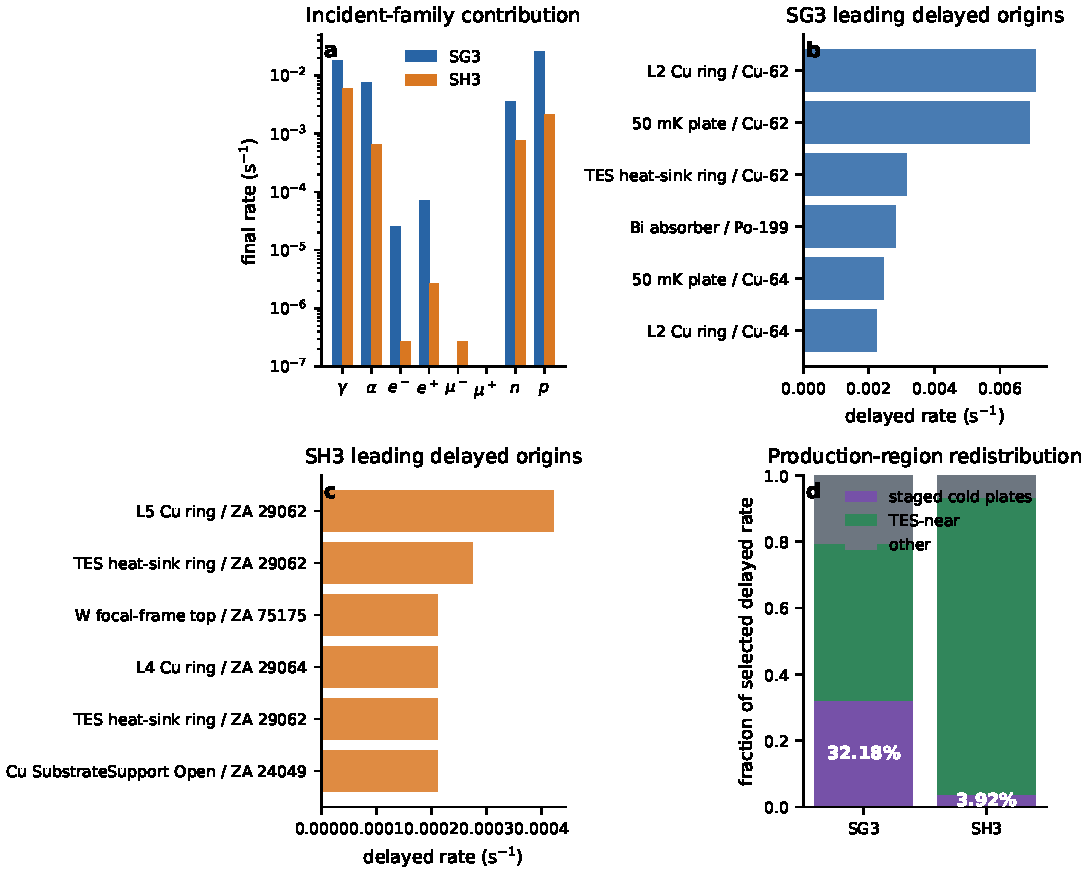
\includegraphics[width=0.98\linewidth]{figures/fig08_background_origins.pdf}
\caption{Selected background origins in the matched SG3 and SH3 catalogues.
(a) Final direct rate by incident family. (b,c) Leading SG3 and SH3 delayed
source-volume/parent-nuclide groups. (d) Selected delayed rate grouped into
staged cold plates, TES-near structures, and other structures. Moving the focal
plane into the chimney reduces the staged-cold-region share from 32.18\% to
3.92\%.}
\label{fig:background_origin_story}
\end{figure}

The family decomposition changes the physical interpretation of the reference
background. Prompt leakage is supported only by the broadband gamma sample,
whereas proton-induced delayed activity is the largest direct component. The
leading SG3 delayed groups are $^{62}$Cu in the L2 copper support ring and the
50 mK mixing-chamber plate, followed by the TES heat-sink ring and the bismuth
absorber. Thus total inventory alone is insufficient: the relevant quantity is
the activity that is both produced in a geometrically coupled location and
selected in the science window.

The production-region view makes the geometry lever explicit. In SG3,
$32.18\%$ of the selected delayed rate originates in the DR/mixing-chamber and
staged cold plates and another $47.29\%$ in TES-near structures. The SH3
translation removes the focal plane from the direct cold-stage projection; the
corresponding staged-cold-region fraction is $3.92\%$, while the selected delayed
rate falls from $3.82661\times10^{-2}$ to $3.62467\times10^{-3}\cps$.

\FloatBarrier

\subsection{Final side-chimney active-shield geometry}
\label{subsec:optimized_shield_results}

The final SH3 geometry places the six TES layers along the lateral chimney axis
at $z'=-2.80$ cm. A 3 mm aluminium wall joins the chimney continuously to the DR;
the chimney bottom remains 0.25 cm above the DR bottom. A compact tungsten frame
supports the focal plane, and three active BGO volumes cover the chimney side,
the front optical annulus, and the rear cold-port annulus. Figure~\ref{fig:optimized_shield_background}
connects this layout to the cut-flow and final composition, while
Table~\ref{tab:final_geometry} records the dimensions used by the transport.

\begin{figure}[!ht]
\centering
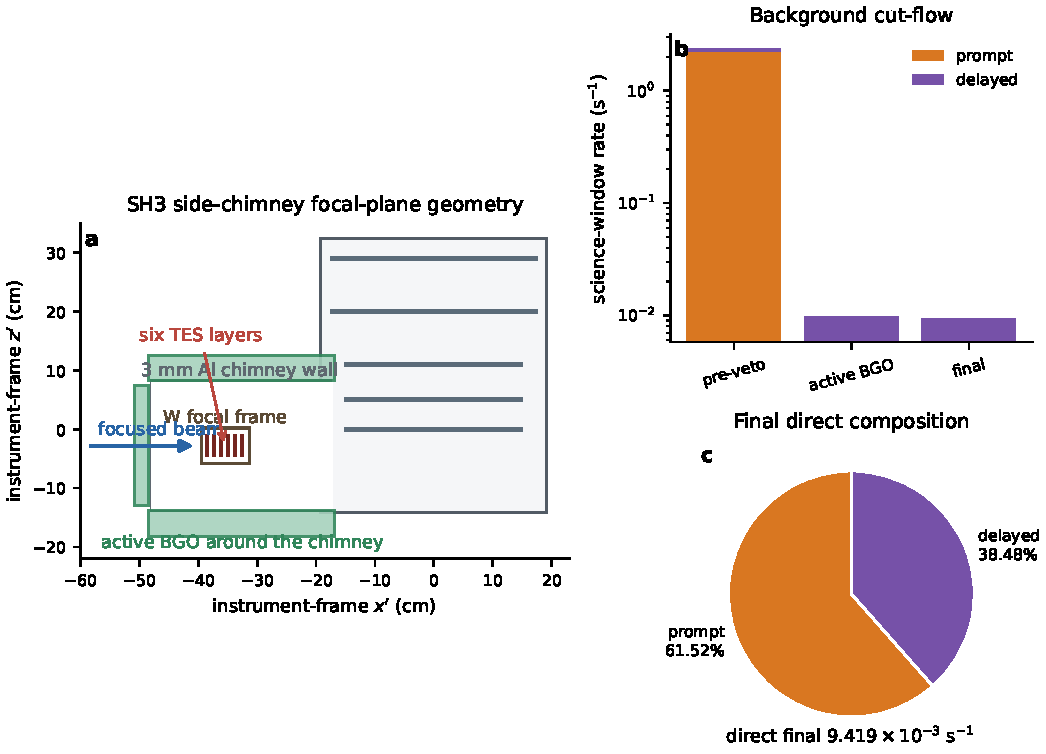
\includegraphics[width=0.92\linewidth]{figures/fig09_sh3_geometry_background.pdf}
\caption{SH3 chimney geometry and selected background. (a) Instrument-frame
section showing the lateral aluminium chimney, six TES layers, tungsten focal
frame, focused beam, staged cold plates, and active BGO. (b) Prompt and delayed
direct rates through the science-window, active-BGO, and final-topology stages.
(c) Composition of the final direct background
($9.41868\times10^{-3}\cps$).}
\label{fig:optimized_shield_background}
\end{figure}

\begin{table}[!ht]
\centering
\caption{Final SH3 side-chimney geometry in local instrument coordinates.}
\label{tab:final_geometry}
\footnotesize
\begin{tabular}{p{0.23\linewidth}p{0.34\linewidth}p{0.34\linewidth}}
\toprule
Element & Final setting & Physical role \\
\midrule
Aluminium chimney & inner/outer radius 10.75/11.05 cm; 3 mm wall & laterally separates the TES from the staged cold region \\
Common axis and clearance & $z'=-2.80$ cm; chimney/DR bottoms $-13.85/-14.10$ cm & continuous welded interface with 0.25 cm clearance \\
TES focal plane & six Ta-pixel layers along the chimney axis & preserves the detector response and multilayer stopping depth \\
Tungsten focal frame & outer/inner square 6.00/5.40 cm; depth 2.00 cm & compact local support and aperture definition \\
Cold-stage/optical ports & 1.50 cm cold ports; 6.00 cm upper optical cut & retains thermal services and focused-beam access \\
Active BGO & side shield, front optical annulus, rear cold-port annulus & event-by-event anticoincidence around the chimney \\
BGO threshold & 50 keV offline deposited energy; 80 keV native trigger reference & common active-veto decision \\
\bottomrule
\end{tabular}
\end{table}

The selected-area comparison verifies that this displacement does not trade away
the optical response. SG3 gives $15.12324\pm0.04492\,\mathrm{cm^2}$ and SH3 gives
$15.08544\pm0.04503\,\mathrm{cm^2}$ after final selection, so the chimney
retains $99.75\%$ of the reference effective area.

\FloatBarrier

\subsection{Full-chain background and statistical support}
\label{subsec:optimized_fullchain}

Table~\ref{tab:optimized_cutflow} follows the SH3 streams through the same
response and event sequence. The background rates in this table are direct
no-coincidence values; the mission calculation applies the measured common-time
factor at every trajectory node.

\begin{table}[!ht]
\centering
\caption{SH3 response-convolved science-window cut-flow. Background entries are
direct no-coincidence counts/rates; signal entries give counts/effective area.}
\label{tab:optimized_cutflow}
\footnotesize
\begin{tabular}{lccc}
\toprule
Stream & Pre-veto & After active BGO & Final topology/FoV \\
\midrule
Prompt background & 3212 / $2.23515\cps$ & 12 / $5.79401\times10^{-3}\cps$ & 12 / $5.79401\times10^{-3}\cps$ \\
Delayed activation & 3249 / $0.127481\cps$ & 122 / $4.01926\times10^{-3}\cps$ & 111 / $3.62467\times10^{-3}\cps$ \\
Total background & 6461 / $2.36263\cps$ & 134 / $9.81327\times10^{-3}\cps$ & 123 / $9.41868\times10^{-3}\cps$ \\
Focused signal & 28434 / $15.35436\,\mathrm{cm^2}$ & 28434 / $15.35436\,\mathrm{cm^2}$ & 27936 / $15.08544\,\mathrm{cm^2}$ \\
\bottomrule
\end{tabular}
\end{table}

Active BGO reduces the total direct rate to $0.4154\%$ of its pre-veto value.
The topology test then retains $95.98\%$ of the BGO-selected rate. Prompt gamma
contributes $5.79401\times10^{-3}\cps$ (61.52\%) and delayed activation
$3.62467\times10^{-3}\cps$ (38.48\%). The day-15 common-time background is
$9.280\times10^{-3}\cps$, which is the value used for the primary mission
projection.

\begin{table}[!ht]
\centering
\caption{Finite-transport support of the SH3 final direct background. Intervals
are two-sided 95\% Garwood count intervals scaled by the component event weight;
subtotal upper endpoints are diagnostics, not joint confidence intervals.}
\label{tab:optimized_component_precision}
\scriptsize
\resizebox{\linewidth}{!}{%
\begin{tabular}{lrrrrr}
\toprule
Component & Records & Weight / $\cps$ & Central rate / $\cps$ & 95\% interval / $\cps$ & Total / \% \\
\midrule
Prompt $\alpha$ & 0 & $5.4193\times10^{-3}$ & 0 & $[0,1.9991\times10^{-2}]$ & 0 \\
Prompt $e^-$ & 0 & $1.8840\times10^{-3}$ & 0 & $[0,6.9500\times10^{-3}]$ & 0 \\
Prompt $e^+$ & 0 & $5.4388\times10^{-3}$ & 0 & $[0,2.0063\times10^{-2}]$ & 0 \\
Prompt $\gamma$ & 12 & $4.8283\times10^{-4}$ & $5.7940\times10^{-3}$ & $[2.9939\times10^{-3},1.0121\times10^{-2}]$ & 61.516 \\
Prompt $\mu^-$ & 0 & $1.3461\times10^{-3}$ & 0 & $[0,4.9655\times10^{-3}]$ & 0 \\
Prompt $\mu^+$ & 0 & $3.9779\times10^{-3}$ & 0 & $[0,1.4674\times10^{-2}]$ & 0 \\
Prompt $n$ & 0 & $5.5440\times10^{-3}$ & 0 & $[0,2.0451\times10^{-2}]$ & 0 \\
Prompt $p$ & 0 & $1.2360\times10^{-2}$ & 0 & $[0,4.5595\times10^{-2}]$ & 0 \\
Prompt subtotal & 12 & -- & $5.7940\times10^{-3}$ & upper sum $1.4281\times10^{-1}$ & 61.516 \\
Delayed $\alpha$ & 19 & $3.4284\times10^{-5}$ & $6.5139\times10^{-4}$ & $[3.9218\times10^{-4},1.0172\times10^{-3}]$ & 6.916 \\
Delayed $e^-$ & 1 & $2.6633\times10^{-7}$ & $2.6633\times10^{-7}$ & $[6.7429\times10^{-9},1.4839\times10^{-6}]$ & 0.003 \\
Delayed $e^+$ & 4 & $6.7536\times10^{-7}$ & $2.7015\times10^{-6}$ & $[7.3606\times10^{-7},6.9168\times10^{-6}]$ & 0.029 \\
Delayed $\gamma$ & 52 & $2.0320\times10^{-6}$ & $1.0567\times10^{-4}$ & $[7.8917\times10^{-5},1.3857\times10^{-4}]$ & 1.122 \\
Delayed $\mu^-$ & 4 & $6.8409\times10^{-8}$ & $2.7364\times10^{-7}$ & $[7.4557\times10^{-8},7.0062\times10^{-7}]$ & 0.003 \\
Delayed $\mu^+$ & 0 & $3.9662\times10^{-9}$ & 0 & $[0,1.4631\times10^{-8}]$ & 0 \\
Delayed $n$ & 11 & $6.8532\times10^{-5}$ & $7.5385\times10^{-4}$ & $[3.7632\times10^{-4},1.3488\times10^{-3}]$ & 8.004 \\
Delayed $p$ & 20 & $1.0553\times10^{-4}$ & $2.1105\times10^{-3}$ & $[1.2892\times10^{-3},3.2595\times10^{-3}]$ & 22.408 \\
Delayed subtotal & 111 & -- & $3.6247\times10^{-3}$ & upper sum $5.7733\times10^{-3}$ & 38.484 \\
\midrule
Total background & 123 & -- & $9.4187\times10^{-3}$ & component upper sum $1.4858\times10^{-1}$ & 100.000 \\
\bottomrule
\end{tabular}}
\end{table}

The component table exposes where finite transport support remains sparse, but
the primary flux-threshold uncertainty is not obtained by adding its interval
endpoints. The matched delta-method budget gives an 18.67\% relative background
transport term, a 1.13\% timeline term, a 0.30\% selected-area term, and a
negligible accidental-probe term. Their propagation gives a 9.36\% relative
$1\sigma$ uncertainty on the SH3 Gaussian $3\sigma$ flux threshold.

\FloatBarrier

\subsection{Mission performance of the final geometry}
\label{subsec:final_mission_performance}

Figure~\ref{fig:optimized_mission_significance} compares the matched 81-node
folds. At 20 d, SG3 accumulates 1635.07 signal and 86806.00 background counts,
whereas SH3 accumulates 1678.14 and 15551.68. The resulting Gaussian
significances are 5.55 and 13.46; the Asimov values are 5.53 and 13.22.

\begin{figure}[!ht]
\centering
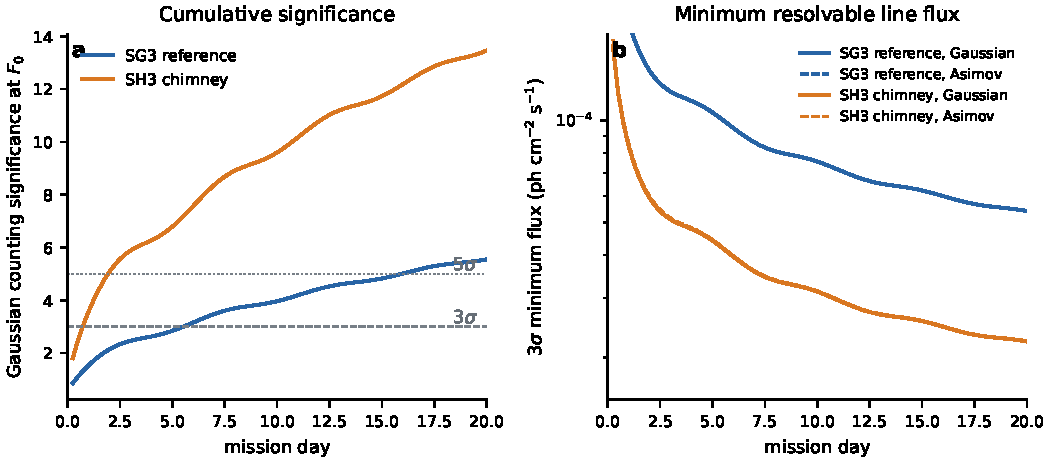
\includegraphics[width=0.98\linewidth]{figures/fig10_mission_performance.pdf}
\caption{Matched 81-node mission performance for the SG3 reference and SH3
chimney geometries. (a) Gaussian counting significance at
$F_0=10^{-4}\phcms$; horizontal lines mark $3\sigma$ and $5\sigma$. (b)
Gaussian and Asimov $3\sigma$ minimum resolvable flux. Both curves use the same
source, response, selection, timing, and atmospheric-transmission contracts.}
\label{fig:optimized_mission_significance}
\end{figure}

\begin{table}[!ht]
\centering
\caption{Matched mission projection for the SG3 reference and SH3 chimney
geometries. Parentheses give the propagated $1\sigma$ statistical uncertainty of
the Gaussian $3\sigma$ flux threshold.}
\label{tab:primary_sensitivity}
\footnotesize
\resizebox{\linewidth}{!}{%
\begin{tabular}{lrr}
\toprule
Quantity & SG3 reference & SH3 chimney \\
\midrule
Selected effective area / $\mathrm{cm^2}$ & $15.12324\pm0.04492$ & $15.08544\pm0.04503$ \\
Day-15 background / $\cps$ & $5.12802\times10^{-2}$ & $9.2800\times10^{-3}$ \\
Day-15 signal at $F_0$ / $\cps$ & $9.53616\times10^{-4}$ & $9.79040\times10^{-4}$ \\
20 d background counts & 86806.00 & 15551.68 \\
20 d signal counts at $F_0$ & 1635.07 & 1678.14 \\
$Z_{20\mathrm d}$, Gaussian / Asimov & 5.550 / 5.532 & 13.457 / 13.225 \\
$T_{3\sigma}$, Gaussian / Asimov / d & 5.525 / 5.555 & 0.724 / 0.753 \\
$T_{5\sigma}$, Gaussian / Asimov / d & 15.932 / 16.010 & 1.935 / 2.030 \\
$F_{3\sigma}(20\,\mathrm d)$, Gaussian / Asimov / $\phcms$ &
$(5.406\pm0.401)\times10^{-5}$ / $5.415\times10^{-5}$ &
$(2.229\pm0.209)\times10^{-5}$ / $2.238\times10^{-5}$ \\
\bottomrule
\end{tabular}}
\end{table}

The SH3 background is 18.10\% of the SG3 value while its selected effective area
is 99.75\% of the reference. The Gaussian 20 d minimum flux is 41.24\% of the SG3
threshold, equivalent to a 2.43-fold improvement. The close Gaussian--Asimov
agreement at the endpoint confirms that the comparison is not an artefact of the
large-background approximation.

\section{Discussion}
\label{sec:discussion}

The main result is a connected physical explanation of the geometry change. In
SG3, the TES lies below the staged cold plates, and selected delayed activity from
that region supplies 32.18\% of the delayed science-window rate. SH3 moves the
same six-layer focal plane laterally into a BGO-surrounded chimney, reducing that
share to 3.92\%. The effective area is unchanged within 0.25\%, while the mature
background falls by a factor of 5.53. Geometry, selected-event provenance, and
mission sensitivity are therefore three views of the same result.

This analysis sequence is consistent with recent instrument-background studies.
COSI transports a detailed balloon payload, separates prompt and activation
components, and compares their spectral and temporal behaviour with flight data
\cite{Gallego2025Balloon}. DIXE likewise begins with a detailed TES payload and
asks which incident particles, production regions, and processes make the
detected spectrum \cite{Tian2026DIXE}. Here the distinction between total
inventory and selected-event origin is decisive: the leading selected groups are
localized copper and near-field structures, so designing from total activity
alone would miss the geometric lever.

The final component mix also separates the roles of the instrument layers.
Active BGO supplies the dominant suppression, reducing the SH3 direct
science-window rate from 2.36263 to $9.8133\times10^{-3}\cps$. The permissive
topology test removes a smaller residual while retaining 98.25\% of the
science-window signal. Broadband atmospheric gamma supplies the remaining prompt
term; activation from all eight incident families supplies the delayed term.

The observing role of this telescope is complementary to INTEGRAL/SPI and COSI,
which measure diffuse bulge, disk, and broader Galactic emission
\cite{Siegert2016AA,Kierans2020,Siegert2020COSI,Yoneda2025,Karwin2023}. The
Laue-lens TES concept exchanges sky coverage for a concentrated beam and a
sub-keV window. Its natural targets are compact 511 keV sources, an unresolved
central component, and pointed follow-up observations. The 20 d values in
Table~\ref{tab:primary_sensitivity} quantify that continuously observed,
narrow-line reference case.

\subsection{Scope and next steps}
\label{subsec:limitations}

The mission values are statistical projections for the detector--cryostat
geometries and the synthetic, continuously on-source trajectory. They use a
50 keV offline BGO deposited-energy threshold, a detector-level topology test, all eight
prompt families, and all eight activation families. The BGO criterion is an
ideal deposited-energy threshold rather than a measured hardware trigger
efficiency. Background from the Laue optics and balloon platform lies outside the
detector--cryostat budget. Radiation-field, cross-section, calibration,
reconstruction, and pointing systematics are also outside the propagated
statistical uncertainty.

The current precision is limited mainly by the finite number and unequal weights
of selected transport events. Future validation should increase the prompt-gamma
and dominant delayed-family support, repeat production-position sampling to test
spatial convergence, replace the synthetic trajectory with a flight plan and
visibility history, and calibrate the energy response and BGO trigger efficiency.
A spatial--spectral likelihood can then use the focused spot and control regions
while profiling background nuisance parameters \cite{Cowan2011}. This extends
the present source-to-geometry logic without changing the closed SG3--SH3
comparison.

\subsection{Conclusions}
\label{sec:conclusions}

The SG3 reference identifies the staged cold region and nearby activated
structures as a major source of selected delayed background. Relocating the
six-layer TES focal plane into the SH3 lateral chimney reduces the cold-stage
share from 32.18\% to 3.92\% while retaining $99.75\%$ of the selected effective
area. At day 15, SH3 gives $B=9.280\times10^{-3}\cps$ and
$S=9.790\times10^{-4}\cps$ at $F_0=10^{-4}\phcms$. Along the fixed-$45^\circ$
20 d trajectory it reaches Gaussian and Asimov significances of 13.46 and 13.22,
with a Gaussian $3\sigma$ threshold of
$(2.229\pm0.209)\times10^{-5}\phcms$. The matched threshold improves by about
2.43 relative to SG3, demonstrating how particle-, nuclide-, and
position-resolved background information can be converted into a focal-plane
geometry and a mission-scale 511 keV performance prediction.

\section*{Data and software availability}
Before publication, a versioned public repository or institutional archive should provide the geometry and source definitions, stochastic-analysis conventions, analysis and figure-generation scripts, LaTeX source, and derived validation products needed to reproduce the tables and figures in this paper.

\section*{Declarations}
\textbf{Funding} To be completed before journal submission.

\textbf{Competing interests} To be completed before journal submission.

\textbf{Author contributions} To be completed before journal submission.

\textbf{Ethics approval and consent to participate} Not applicable.

\begin{thebibliography}{99}

\bibitem{Prantzos2011}
N. Prantzos, C. Boehm, A.M. Bykov, R. Diehl, K. Ferriere, N. Guessoum, P. Jean, J. Knoedlseder, A. Marcowith, I.V. Moskalenko, A. Strong, G. Weidenspointner, The 511 keV emission from positron annihilation in the Galaxy, Rev. Mod. Phys. 83 (2011) 1001--1056, doi:10.1103/RevModPhys.83.1001.

\bibitem{Jean2006}
P. Jean, J. Knoedlseder, V. Lonjou, M. Allain, J.-P. Roques, G.K. Skinner, B.J. Teegarden, G. Vedrenne, P. von Ballmoos, B. Cordier, P. Caraveo, R. Diehl, P. Durouchoux, P. Leleux, R. Schanne, G. Weidenspointner, Spectral analysis of the Galactic $e^+e^-$ annihilation emission, Astron. Astrophys. 445 (2006) 579--589, doi:10.1051/0004-6361:20053765.

\bibitem{Kierans2020}
C.A. Kierans, S.E. Boggs, A. Zoglauer, A.W. Lowell, C. Sleator, J. Beechert, T.J. Brandt, P. Jean, H. Lazar, J. Roberts, T. Siegert, J.A. Tomsick, P. von Ballmoos, Detection of the 511 keV Galactic positron annihilation line with COSI, Astrophys. J. 895 (2020) 44, doi:10.3847/1538-4357/ab89a9.

\bibitem{Siegert2016AA}
T. Siegert, R. Diehl, G. Khachatryan, M.G.H. Krause, F. Guglielmetti, J. Greiner, A.W. Strong, X. Zhang, Gamma-ray spectroscopy of positron annihilation in the Milky Way, Astron. Astrophys. 586 (2016) A84, doi:10.1051/0004-6361/201527510.

\bibitem{Siegert2016V404}
T. Siegert, R. Diehl, J. Greiner, M.G.H. Krause, A.M. Beloborodov, M. Cadolle Bel, F. Guglielmetti, J. Rodriguez, A.W. Strong, X. Zhang, Positron annihilation signatures associated with the outburst of the microquasar V404 Cygni, Nature 531 (2016) 341--343, doi:10.1038/nature16978.

\bibitem{Knodlseder2005AllSky}
J. Knoedlseder, P. Jean, V. Lonjou, G. Weidenspointner, N. Guessoum, R. Diehl, W. Gillard, M.J. Harris, G.K. Skinner, P. von Ballmoos, G. Vedrenne, P. Caraveo, B. Cordier, V. Schoenfelder, B.J. Teegarden, The all-sky distribution of 511 keV electron-positron annihilation emission, Astron. Astrophys. 441 (2005) 513--532, doi:10.1051/0004-6361:20042063.

\bibitem{Yoneda2025}
H. Yoneda, T. Siegert, S. Mittal, Imaging the positron annihilation line with 20 years of INTEGRAL/SPI observations, arXiv:2509.01066, 2025.

\bibitem{Siegert2020COSI}
T. Siegert, S.E. Boggs, J.A. Tomsick, A.C. Zoglauer, C.A. Kierans, C.C. Sleator, J. Beechert, T.J. Brandt, P. Jean, H. Lazar, A.W. Lowell, J.M. Roberts, P. von Ballmoos, Imaging the 511 keV positron annihilation sky with COSI, Astrophys. J. 897 (2020) 45, doi:10.3847/1538-4357/ab9607.

\bibitem{Siegert2019Kinematics}
T. Siegert, R. Diehl, G. Khachatryan, M.G.H. Krause, F. Guglielmetti, J. Greiner, A.W. Strong, X. Zhang, Constraints on positron annihilation kinematics in the inner Galaxy, Astron. Astrophys. 627 (2019) A126, doi:10.1051/0004-6361/201833856.

\bibitem{DeCesare2011}
G. De Cesare, Searching for the 511 keV annihilation line from galactic compact objects with the IBIS gamma ray telescope, Astron. Astrophys. 531 (2011) A56, doi:10.1051/0004-6361/201116516.

\bibitem{Barriere2009Laue}
N.M. Barriere, L. Natalucci, N. Abrosimov, P. von Ballmoos, P. Bastie, P. Courtois, M. Jentschel, J. Knodlseder, J. Rousselle, P. Ubertini, Soft gamma-ray optics: new Laue lens design and performance estimates, arXiv:0910.0488, 2009.

\bibitem{Barriere2011LauePrototype}
N.M. Barriere, J.A. Tomsick, S.E. Boggs, A. Lowell, P. von Ballmoos, Developing a second generation Laue lens prototype: high reflectivity crystals and accurate assembly, arXiv:1111.6700, 2011.

\bibitem{Weidenspointner2006MAX}
G. Weidenspointner, C.B. Wunderer, N. Barriere, A. Zoglauer, P. von Ballmoos, Monte Carlo study of detector concepts for the MAX Laue Lens gamma-ray telescope, arXiv:astro-ph/0603152, 2006.

\bibitem{Shirazi2023}
F. Shirazi, E. Gau, M.A. Hossen, D. Becker, D. Schmidt, D. Swetz, D. Bennett, D. Braun, F. Kislat, J. Gard, J. Mates, J. Weber, N.R. Cavero, S. Chun, L. Lisalda, A. West, B. Dev, F. Ferrer, R. Bose, J. Ullom, H. Krawczynski, The 511-CAM Mission: A pointed 511 keV gamma-ray telescope with a focal plane detector made of stacked transition edge sensor microcalorimeter arrays, J. Astron. Telesc. Instrum. Syst. 9 (2023) 024006, doi:10.1117/1.JATIS.9.2.024006.

\bibitem{Zhang2022TESGamma}
S. Zhang, J.-K. Xia, T. Sun, et al., Transition edge sensor based detector: from X-ray to gamma-ray, arXiv:2204.00010, 2022.

\bibitem{Hu2026}
K. Hu, M. Fritts, D. Becker, D. Schmidt, F. Zhou, A. Dasgupta, F. Kislat, M. Keller, S. Chun, A.G. Detoito, E. Gau, X. Jin, D. Bennett, D. Braun, J. Gard, J.A.B. Mates, J. Nobles, D. Radomski, N. Rodriguez Cavero, R. Snodgrass, D. Swetz, J. Ullom, S. Vengalil Menon, J. Weber, K. Wimalasena, H. Krawczynski, Design of a mission to measure the shape and substructure of the 511 keV gamma-ray line from the center of the Milky Way, J. Astron. Telesc. Instrum. Syst. 12 (2026) 025002, doi:10.1117/1.JATIS.12.2.025002.

\bibitem{Gallego2025Balloon}
S. Gallego, U. Oberlack, J. Lommler, C.M. Karwin, A. Zoglauer, P. Jean, P. von Ballmoos, C. Kierans, C.C. Sleator, J.A. Tomsick, S.E. Boggs, Bottom-up background simulations of the 2016 COSI balloon flight, Astrophys. J. 986 (2025) 116, doi:10.3847/1538-4357/add6a0.

\bibitem{Tian2026DIXE}
R. Tian, J. Mao, J. Liu, H. Jin, W. Cui, Simulation of non-X-ray background for the DIffuse X-ray Explorer (DIXE) mission, arXiv:2604.13569, 2026.

\bibitem{Caputo2017}
R. Caputo, F. Kislat, J. Racusin, on behalf of the AMEGO Team, AMEGO: Simulations of the instrument performance, Proc. 35th International Cosmic Ray Conference, PoS(ICRC2017) 783 (2018), doi:10.22323/1.301.0783.

\bibitem{Gottardi2021TESReview}
L. Gottardi, K. Nagayoshi, A review of X-ray microcalorimeters based on superconducting transition edge sensors for astrophysics and particle physics, Applied Sciences 11 (2021) 3793, doi:10.3390/app11093793.

\bibitem{Xie2026AlMn}
L. Xie, Y. Zhang, Z. Li, Z. Liu, S. Shu, J. Zhou, X. Li, H. Li, H. Gao, Y. Gu, X. Lu, Y. Zhao, C. Liu, Beyond one-thousandth energy resolution with an AlMn TES detector, arXiv:2602.11728, 2026.

\bibitem{Vavagiakis2017AlMnMagnetic}
E.M. Vavagiakis, S.W. Henderson, K. Zheng, H.-M. Cho, N.F. Cothard, B. Dober, S.M. Duff, P.A. Gallardo, G. Hilton, J. Hubmayr, K.D. Irwin, B.J. Koopman, D. Li, F. Nati, M.D. Niemack, C.D. Reintsema, S. Simon, J.R. Stevens, A. Suzuki, B. Westbrook, Magnetic sensitivity of AlMn TESes and shielding considerations for next-generation CMB surveys, arXiv:1710.08456, 2017.

\bibitem{NISTXCOM}
J.H. Hubbell, S.M. Seltzer, XCOM: Photon Cross Section Database, NIST Standard Reference Database 8 (XGAM), National Institute of Standards and Technology, doi:10.18434/T48G6X.

\bibitem{Sturner2003}
S.J. Sturner, C.R. Shrader, G. Weidenspointner, B.J. Teegarden, D. Attie, B. Cordier, R. Diehl, C. Ferguson, P. Jean, A. von Kienlin, P. Paul, F. Sanchez, S. Schanne, P. Sizun, G. Skinner, C.B. Wunderer, Monte Carlo simulations and generation of the SPI response, Astron. Astrophys. 411 (2003) L81--L84, doi:10.1051/0004-6361:20031171.

\bibitem{Agostinelli2003}
S. Agostinelli, J. Allison, K. Amako, et al., Geant4---a simulation toolkit, Nucl. Instrum. Methods Phys. Res. A 506 (2003) 250--303, doi:10.1016/S0168-9002(03)01368-8.

\bibitem{Allison2016}
J. Allison, K. Amako, J. Apostolakis, et al., Recent developments in Geant4, Nucl. Instrum. Methods Phys. Res. A 835 (2016) 186--225, doi:10.1016/j.nima.2016.06.125.

\bibitem{SanchezDelRio2011XOP}
M. Sanchez del Rio, R.J. Dejus, XOP v2.4: recent developments of the x-ray optics software toolkit, Proc. SPIE 8141 (2011) 814115, doi:10.1117/12.893911.

\bibitem{Guan2023BraggReflection}
F. Guan, M. Asai, D.A. Bartkoski, M. Kleckner, Z. Harel, M. Salehpour, Adding the X-ray Bragg reflection physical process in crystal to the Geant4 Monte Carlo simulation toolkit, part I: reflection from a crystal slab, Precision Radiation Oncology 7(1) (2023) 59--66.

\bibitem{Reiazi2025G4BraggReflection}
R. Reiazi, D. Lee, D. Bartkoski, M. Kleckner, M. Salehpour, G4BraggReflection for accurate modeling of Bragg reflection in perfect and mosaic crystals, J. Phys. D: Appl. Phys. 58 (2025) 295102, doi:10.1088/1361-6463/aded1d.

\bibitem{Zoglauer2006}
A. Zoglauer, R. Andritschke, F. Schopper, MEGAlib: The Medium Energy Gamma-ray Astronomy Library, New Astron. Rev. 50 (2006) 629--632, doi:10.1016/j.newar.2006.06.049.

\bibitem{Sato2015EXPACS}
T. Sato, Analytical model for estimating terrestrial cosmic ray fluxes nearly anytime and anywhere in the world: extension of PARMA/EXPACS, PLoS ONE 10 (2015) e0144679, doi:10.1371/journal.pone.0144679.

\bibitem{Sato2016PARMA4}
T. Sato, Analytical model for estimating the zenith angle dependence of terrestrial cosmic ray fluxes, PLoS ONE 11 (2016) e0160390, doi:10.1371/journal.pone.0160390.

\bibitem{Mahoney1981Atmospheric}
W.A. Mahoney, J.C. Ling, A.S. Jacobson, HEAO 3 measurements of the atmospheric positron annihilation line, J. Geophys. Res. 86 (1981) 11098--11104, doi:10.1029/JA086iA13p11098.

\bibitem{Harris2003Atmospheric}
M.J. Harris, G.H. Share, M.D. Leising, Spatial and temporal variability of the gamma radiation from Earth's atmosphere during a solar cycle, J. Geophys. Res. Space Phys. 108 (2003) 1435, doi:10.1029/2003JA009958.

\bibitem{Kondev2021NUBASE}
F.G. Kondev, M. Wang, W.J. Huang, S. Naimi, G. Audi, The NUBASE2020 evaluation of nuclear physics properties, Chinese Phys. C 45 (2021) 030001, doi:10.1088/1674-1137/abddae.

\bibitem{Kierans2017}
C.A. Kierans, S.E. Boggs, J.-L. Chiu, A. Lowell, C. Sleator, J.A. Tomsick, A. Zoglauer, M. Amman, H.-K. Chang, C.-H. Tseng, C.-Y. Yang, C.-H. Lin, P. Jean, P. von Ballmoos, The 2016 Super Pressure Balloon flight of the Compton Spectrometer and Imager, arXiv:1701.05558, 2017.

\bibitem{Karwin2023}
C.M. Karwin, T. Siegert, J. Beechert, J.A. Tomsick, T.A. Porter, M. Negro, C. Kierans, M. Ajello, I. Martinez Castellanos, A. Shih, A. Zoglauer, S.E. Boggs, Probing the Galactic diffuse continuum emission with COSI, arXiv:2310.12206, 2023.

\bibitem{Cowan2011}
G. Cowan, K. Cranmer, E. Gross, O. Vitells, Asymptotic formulae for likelihood-based tests of new physics, Eur. Phys. J. C 71 (2011) 1554, doi:10.1140/epjc/s10052-011-1554-0.

\end{thebibliography}
\end{document}
